%%{ DOC HEAD

\pdfoutput=1
\documentclass[a4paper,11pt,titlepage,twoside]{book}

\usepackage[english]{babel}
\usepackage[utf8]{inputenc}
\usepackage{csquotes}

\usepackage{amsmath,amsfonts,amssymb,bm}
\usepackage{nicefrac}

\usepackage{algorithm,algpseudocode}
\usepackage[title,titletoc]{appendix}
\usepackage{latexsym}
\usepackage{a4wide}
\usepackage{color}
\usepackage{indentfirst}
\usepackage{graphicx}       %%% graphics for dvips
\usepackage{fancyhdr,lastpage}
\usepackage{longtable}
\usepackage{pifont}
\usepackage{makeidx}
\usepackage{multirow}
\usepackage{dcolumn}
\usepackage{epstopdf}
\usepackage{url}
\usepackage{listings}
\usepackage{relsize}
\usepackage{pdfpages}
\usepackage{url}
\usepackage{lipsum}
\usepackage{isotope}
\usepackage{verbatim}
\usepackage{xcolor}
\usepackage{tcolorbox}
\usepackage{subfig} % subfloat
\usepackage[export]{adjustbox}

%%{ tikz

\usepackage{tikz}
\usepackage{pgfplots}
\pgfplotsset{compat=1.14}
\usetikzlibrary{backgrounds,arrows,automata,shapes,positioning,calc,through,spy}
\pgfdeclarelayer{background}
\pgfdeclarelayer{foreground}
\pgfsetlayers{background,main,foreground}

\tikzset{
    imgletter/.style={
      rectangle,
      inner sep=2pt,
      rounded corners=.1em,
      text=black,
      minimum height=1em,
      text centered,
      fill=white,
      fill opacity=1.0,
      text opacity=1,
      anchor=south west,
  },
}

%%}

% \newcommand{\includepaper}[1]{\includepdf[scale=0.85,pages=-,pagecommand={\thispagestyle{plain}}]{./papers_to_include_pdf/#1}}
% \newcommand{\includepaper}[1]{\conditionalClearPage \fullciteinbox{#1}{Here will be the pdf of the paper}}
\newcommand{\includepaper}[1]{\fullciteinbox{#1}{Here will be the pdf of the paper}}

%%{ fullcite box

\definecolor{light-gray}{gray}{0.95}
\newcommand{\fullciteinbox}[2]{%

\DeclareCiteCommand{\fullcite}
{\usebibmacro{prenote}}
{\clearfield{addendum}%
  \usedriver
  {\defcounter{minnames}{6}%
  \defcounter{maxnames}{6}}
{\thefield{entrytype}}}
{\multicitedelim}
{\usebibmacro{postnote}}

%\vspace{3em}%
%\raisebox{3em}[3em][3em]{%
% \vspace{-0.2em}
\begin{tcolorbox}[width=\textwidth,colback={light-gray},title={}]%
\ifx&#2&
\else
  \textbf{#2}:\\\\
\fi
\begin{minipage}[t]{0.07\linewidth}%
\raggedright%
\cite{#1}%
\end{minipage}%
\begin{minipage}[t]{0.93\linewidth}%
\fullcite{#1}%
\end{minipage}%
\end{tcolorbox}%
%}%
% \vspace{-0.5em}
}%

%%}

%%{ acronym

\usepackage[nolist,nohyperlinks]{acronym}
\acrodef{GPS}[GPS]{Global Positioning System}
\acrodef{SLAM}[SLAM]{Simultaneous Localization And Mapping}
\acrodef{SLAMs}[SLAMs]{Simultaneous Localization And Mapping systems}
\acrodef{GPS}[GPS]{Global Positioning System}
\acrodef{RTK}[RTK]{Real-time Kinematics}
\acrodef{GNSS}[GNSS]{Global Navigation Satellite System}
\acrodef{ROS}[ROS]{Robot Operating System}
\acrodef{API}[API]{Application Programming Interface}
\acrodef{UAV}[UAV]{Unmanned Aerial Vehicle}
\acrodef{MAV}[MAV]{Micro Aerial Vehicle}
\acrodef{UGV}[UGV]{Unmanned Ground Vehicle}
\acrodef{UV}[UV]{Ultra-Violet}
\acrodef{LED}[LED]{Light-emitting Diode}
\acrodef{MBZIRC}[MBZIRC]{Mohamed Bin Zayed International Robotics Challenge}
\acrodef{DARPA}[DARPA]{Defense Advanced Research Projects Agency}
\acrodef{IMU}[IMU]{Inertial Measurement Unit}
\acrodef{LTI}[LTI]{Linear time-invariant}
\acrodef{MPC}[MPC]{Model Predictive Control}
\acrodef{UVDAR}[UVDAR]{Ultra-Violet Direction And Ranging}
\acrodef{DOF}[DOF]{degree-of-freedom}
\acrodef{DOFs}[DOFs]{degrees-of-freedom}
\acrodef{LiDAR}[LiDAR]{Light Detection and Ranging}
\acrodef{ESC}[ESC]{Electronic Speed Controller}
\acrodef{LKF}[LKF]{Linear Kalman Filter}
\acrodef{UKF}[UKF]{Unscented Kalman Filter}
\acrodef{EKF}[EKF]{Extended Kalman Filter}
\acrodef{RAS}[RAS]{Robotics and Automation Society}
\acrodef{IEEE}[IEEE]{Institute of Electrical and Electronics Engineers}
\acrodef{MRS}[MRS]{Multi-robot Systems Group}
\acrodef{FOV}[FOV]{Field of View}
\acrodef{CdTe}[CdTe]{Cadmium Telluride}
\acrodef{FDNPP}[FDNPP]{Fukushima Daiichi Nuclear Power Plant}

%%}

\usepackage[]{hyperref}

%%{ siunitx

\usepackage{siunitx}
\DeclareSIUnit \parsec {pc}
\DeclareSIUnit \electronvolt {eV}
\DeclareSIUnit \pixel {px}
\DeclareSIUnit \arcmin {arcmin}
\DeclareSIUnit \erg {erg}
\DeclareSIUnit \joul {J}

%%}

% change formatting of lists
\usepackage{enumitem}
\setlist{nosep}
% \setlist{noitemsep}
% how to format particular lists?
% \begin{itemize}[topsep=8pt,itemsep=4pt,partopsep=4pt, parsep=4pt]

% change spacing of the table of contents
% \usepackage{tocloft}
% \renewcommand\cftchapafterpnum{\vskip5pt}
% \renewcommand\cftsecafterpnum{\vskip5pt}

% change formatting of a chapter
\usepackage{titlesec}
\titleformat{\chapter}[block]
{\normalfont\huge\bfseries}{Chapter \thechapter\\\vspace{0.1em}\\}{1em}{\Huge}
% {?}{before}{after}
\titlespacing*{\chapter}{0pt}{-1em}{2em}

\hyphenation{}

%%{ BIBLATEX

\usepackage[backend=bibtex,defernumbers=true,style=ieee,sorting=ydnt,sortcites=true]{biblatex}

\renewcommand*{\bibfont}{\Font}

% \newcounter{mycounter}
% \setcounter{mycounter}{0}
% \newcounter{unrelatedcount}
% \setcounter{unrelatedcount}{0}
% \newcounter{totalcounter}
% \setcounter{totalcounter}{0}

% % Print labelnumbers with suffixes, adjust secondary labelnumber 1/2 (start new numbering of my publications)
% \makeatletter
% \AtDataInput{%
%   \ifkeyword{mine}
%   {
%     \addtocounter{mycounter}{1}
%   }
%   {}
%   \addtocounter{totalcounter}{1}
% }
% \makeatother

% Print labelnumbers with suffixes, adjust secondary labelnumber 2/2
\DeclareFieldFormat{labelnumber}{%
  \ifkeyword{mine}
    {\ifkeyword{core}
      {{\number\numexpr#1}c}%
      {{\number\numexpr#1}a}%
    }%
    {#1}%
}

% {{\number\numexpr#1-\value{bbx:primcount}}a}

\addbibresource{main.bib}

\defbibenvironment{favoritebib}
{\itemize}
{\enditemize}
{\item}

%%}

%%{ CUSTOM MACROS

%%%%%%%%%%%%%%% changemargin environment begin %%%%%%%%%%%%%%%%%%%%%%%%%
\def\changemargin#1#2{\list{}{\rightmargin#2\leftmargin#1}\item[]}
\let\endchangemargin=\endlist
%%%%%%%%%%%%%%% changemargin environment end %%%%%%%%%%%%%%%%%%%%%%%%%

\newcommand{\strong}[1]{\textbf{#1}}
\newcommand{\coord}[1]{\textbf{#1}}
\newcommand{\norm}[1]{\left\lvert#1\right\rvert}
\newcommand{\m}[1]{\ensuremath{\mathbf{#1}}}
\newcommand\numberthis{\addtocounter{equation}{1}\tag{\theequation}}
\newcommand{\corrected}[1]{{\color{black} {#1}}}
% \newcommand{\comment}[1]{{\color{blue} {#1}}}
\newcommand{\add}[1]{{\color{green} {#1}}}
\newcommand{\todo}[1]{{\color{red} TODO {#1}}}
\newcommand{\updated}[1]{{\color{blue} {#1}}}
\newcommand{\reffig}[1]{Fig.~\ref{#1}}
\newcommand{\refalg}[1]{Alg.~\ref{#1}}
\newcommand{\refsec}[1]{Sec.~\ref{#1}}
\newcommand{\reftab}[1]{Table~\ref{#1}}
\newcommand{\real}{\mathbb{R}}
\newcommand{\red}[1]{{\color{red} #1}}
\newcommand{\minus}{\scalebox{0.75}[1.0]{$-$}}
\newcommand{\plus}{\scalebox{0.8}[0.8]{$+$}}
\newcommand{\figvspace}{\vspace{-1em}} % this may eventually do something, so far just a placeholder

\newcommand{\chapternoclear}[1]{
  \begingroup
  \let\cleardoublepage\clearpage
  \chapter{#1}
  \endgroup
}

\newcommand{\conditionalClearPage}{
  \ifdefined\printversion
  %\newpage{}
  %\thispagestyle{empty}
  \clearemptydoublepage
  %\cleardoublepage{\thispagestyle{empty}}
  \else
  \newpage{}
  \clearpage
  \fi
}

%%}

\newcommand{\Author}{Ing. Tomáš Báča}
\newcommand{\Supervisor}{Ing. Martin Saska, Dr. rer. nat.}
\newcommand{\SupervisorSpecialist}{Ing. Michal Platkevic, Ph.D.}
\newcommand{\Programme}{Electrical Engineering and Information Technology}
\newcommand{\Field}{Artificial Intelligence and Biocybernetics}
\newcommand{\Title}{Cooperative Sensing with Group\\[0.5em]of Unmanned Aerial Vehicles}
\newcommand{\DocName}{Doctoral Thesis}
\newcommand{\Keywords}{Unmanned Aerial Vehicles, Ionizing localization}
\newcommand{\DOCVersion}{0.1}
\newcommand{\Year}{2020}
\newcommand{\Month}{September}
\newcommand{\Date}{\Month~\Year}
\newcommand{\Location}{Prague}

% % altering margins
% \setlength{\oddsidemargin}{+0.5cm}
% \setlength{\evensidemargin}{-0.5cm}

% ??
\def\clinks{false}

% listings
\lstset{breaklines=true,captionpos=b,frame=single,language=sh,float=h}
\lstloadlanguages{sh,c}
\def\lstlistingname{Listing}
\def\lstlistlistingname{Listings}

% European layout (no extra space after `.')
\frenchspacing

% no indent, free space between paragraphs
\setlength{\parindent}{1cm}
\setlength{\parskip}{1ex plus 0.5ex minus 0.2ex}

% offsets the head down
\setlength{\headheight}{18pt}

% foot line
\renewcommand{\footrulewidth}{0.4pt}

\fancypagestyle{plain}

% clear the default layout
\fancyhead{}
\fancyfoot{}

% page header
\fancyhead[LO]{\leftmark}
\fancyhead[RE]{\rightmark}
\fancyhead[LE,RO]{\thepage/\pageref{LastPage}}

% page footer
\fancyfoot[L]{CTU in Prague}
\fancyfoot[R]{Department of Cybernetics}
\fancyfoot[C]{}

% without it it does not compile!
\let\bibfont\small

%%}

\begin{document}

\begin{titlepage}
\begin{center}

{\Large CZECH TECHNICAL UNIVERSITY IN PRAGUE}
\vskip 10pt

\vskip 8pt
{\Large Faculty of Electrical Engineering}
 
%\vskip 0pt plus 2fill
\vspace{50pt}
{\Huge\bf DISSERTATION THESIS}\\
\vspace{40pt}

\includegraphics[width=10cm]{fig/lev.pdf}

\vspace{40pt}
{\Large\rm \Author } \\
\vspace{20pt}
{\Large\bf \Title}

\vspace{60pt}
{\bf Department of Cybernetics}\\
\vspace{5pt}   
{Thesis supervisor: {\bf \Supervisor}}

\vspace{30pt}
%{\sc Prague 2013}
\end{center}
\end{titlepage}


\conditionalClearPage
%!TEX root = ../main.tex

~\vfill{}

\section*{Acknowledgments}

Firstly, I would like to express my gratitude to my family for providing me with both material and mental support during my studies.
I am grateful that they allowed me to pursue a student and a researcher's path, a career that is not known for its short-term benefits and securities.
Secondly, my thanks go to Martin Saska, my supervisor, and colleague.
I am grateful for his trust he gave me during the founding and the growth of the MRS group.
I also do not take for granted the creative freedom I was given during my studies and work within the group.
I also thank Tomas Krajnik.
Although our paths have diverged, I am grateful you motivated me to apply to the CTU in Prague and later supervised me during my first steps in aerial robotics.
Furthermore, my thanks go to all the present and past members of the MRS group.
The past six years were a \emph{bumpy ride}, and I am grateful that I could make it with you.
Specifically, I would like to thank my colleagues Vojtech Spurny, Daniel Hert, and Robert Penicka, who often \emph{shared the front seats} with me.
My own path would have probably been different without you.

My next thanks go to everyone who allowed me to work on the projects related to radiation dosimetry for space applications.
Successful orchestration of research in space instrumentation is comparably more difficult than research in mobile robotics.
Even though our results might be small in the grand scheme of things, the path towards them was no less difficult given the tight funding and limited know-how.
Among others, I am grateful to Vladimir Daniel (Czech Aerospace Research Institute), Adolf Inneman (Rigaku Innovative Technologies, s.r.o.), Jan Jakubek, and Michal Platkevic (in that time at the Institute of Experimental and Applied Physics, CTU).
Without you, the VZLUSAT-1 nanosatellite project would not have happened.
Moreover, I am grateful to our colleagues at the University of Iowa and at Pennsylvania State University.
Thank you for the opportunity to collaborate, despite the probably asymmetrical gains from the collaboration.
I would like to thank, among others, my colleagues and friends Randall Mc'Entaffer, Ted Schultz, and James Tutt, who went above and beyond with their hospitality during my visits to their laboratories.

During my Ph.D. studies, my work was supported by the Czech Republic taxpayers through a Ph.D. scholarship.
My work had also been supported by the Czech Technical University grants SGS15/157/OHK3/2T/13 and SGS17/187/OHK3/3T/13.
The Ministry of education of the Czech Republic supported the work by grant no. 7AMB16FR017, and no. LH11053, and by OP VVV funded project CZ.02.1.01/0.0/0.0/16\_019/0000765 ``Research Center for Informatics''.
The Czech Science Foundation supported this work through projects no. 17-16900Y, no. 18-10088Y, and no. 20-10280S.
The Technology Agency of the Czech Republic supported this work through project no. FW01010317.
The European Union's Horizon 2020 research and innovation program supported this work under grant agreement No 871479.
The National Grid Infrastructure MetaCentrum provided access to computing and storage facilities under CESNET 569/2015, and LM2015042.
The Khalifa University of Science funded our participation in the MBZIRC 2017 and MBZIRC 2020 competitions that also motivated this work.
The work on the outer space radiation dosimetry and measurements would not be possible without the Technology Agency of the Czech Republic projects no. TA03011329, no. TA04011295, the Czech Science Foundation projects no. GA13-33324S, GJ18-10088Y, and the project MSMT LH14039 of the Ministry of education youth and sports of the Czech Republic.
The work has been done on behalf of Medipix2 and Medipix3 collaborations.

\vspace{2.5cm}


\conditionalClearPage
%!TEX root = ../main.tex
\begin{changemargin}{0.8cm}{0.8cm} 

~\vfill{}

\section*{Copyright}
\vskip 0.5em

This thesis is a compilation of several articles published during my Ph.D. studies.
The included publications are presented in accordance with the copyrights of IEEE, Springer, Elsevier, IOP Publishing, and Wiley for posting the works for internal institutional uses.
The works are protected by the copyrights of respective publishers and can not be further reprinted without the permission of the publishers. 

\vskip 2.5cm

\textsuperscript{\textcopyright} IEEE, 2018, 2019, 2020\\
\textsuperscript{\textcopyright} IOP Publishing, 2018\\
\textsuperscript{\textcopyright} Wiley, 2019\\
\textsuperscript{\textcopyright} Springer, 2020\\
\textsuperscript{\textcopyright} Elsevier, 2020\\
\end{changemargin} 


\conditionalClearPage
%!TEX root = ../main.tex
%~\vfill{}
\begin{changemargin}{0.8cm}{0.8cm} 

%\begin{center}
%{\large \bf Abstract}
%\end{center}
%{\Large \bf Abstract}
\section*{Abstract}
%\vskip 1em

\todo{}

\vskip 1em

{\bf Keywords} \Keywords

\end{changemargin} 


\pagestyle{fancy}

\conditionalClearPage
\tableofcontents

%% | ------------------------ Chapter 1 ----------------------- |

%%{ Introduction

\chapternoclear{Introduction}

%%{ Author's publications

\section{Author's publications}

Related journals:
\cite{baca2018rospix}
\cite{baca2019autonomous}
\cite{spurny2019cooperative}
\cite{saska2017system}
\cite{giernacki2019realtime}
\cite{chudoba2016exploration}
\cite{saska2020formation}
\cite{loianno2018localization}
\cite{petrlik2020robust}
\cite{stibinger2020localization}
\cite{saikin2020wildfire}
\cite{baca2020mrs}
\cite{petracek2020bioinspired}
\cite{kratky2020autonomous2}
\cite{stasinchuk2020multiuav}
\cite{dmytruk2020safe}
\cite{smrcka2020admittance}
\cite{walter2020extinguishing}
\cite{silano2020power}

Related conference papers:
\cite{baca2019timepix}
\cite{baca2018model}
\cite{baca2016embedded}
\cite{baca2017autonomous}
\cite{saska2017documentation}
\cite{spurny2016complex}
\cite{faigl2017onsolution}
\cite{saska2016formations}
\cite{roucek2019darpa}
\cite{baca2020gamma}

Partially-related journals:
\cite{baca2016miniaturized}
\cite{baca2018timepix}
\cite{daniel2019inorbit}
\cite{urban2017vzlusat}

Partially-related conference papers:
\cite{daniel2016terrestrial}
\cite{daniel2017xray}

%%}

%%}

%% | ------------------------ Chapter 2 ----------------------- |

%%{ Contributions and Related Work

\chapternoclear{Contributions and Related Work}

%%}

%% | ------------------------ Chapter 3 ----------------------- |

%%{ Research-focused UAV Platform

\chapternoclear{Research-focused UAV Platform}

Relevant author's publications (will be discussed):
\fullciteinbox{baca2016embedded}{}
\fullciteinbox{baca2019autonomous}{}
\fullciteinbox{spurny2019cooperative}{}

Author's publications to be included in the thesis:
\includepaper{baca2018model}
\includepaper{baca2020mrs}

%%}

%% | ------------------------ Chapter 4 ----------------------- |

%%{ Advances in remote sensing

\chapternoclear{Advances in remote sensing}

Relevant author's publications (will be discussed):

\fullciteinbox{petrlik2020robust}{}
\fullciteinbox{petracek2020bioinspired}{}
\fullciteinbox{kratky2020autonomous2}{}

Author's publications to be included in the thesis:
\includepaper{spurny2019cooperative}
\includepaper{baca2019autonomous}
\includepaper{loianno2018localization}

\subsection{UAV mutual detection and localization}

The system played an integral role in the ongoing research on relatively-localized \ac{UAV} swarms and formations.
Onboard marker-less \ac{UAV} detection and localization were studied in \cite{vrba2020markerless, vrba2019onboard}.
Two approaches to \ac{UAV} detection were proposed, and were experimentally verified with the proposed system: a Convolutional Neural Network-based method, and a system for processing depth-camera images.

Mutual localization of \acp{UAV} within swarms and formations was presented in \cite{walter2017selflocalization, walter2018fast, walter2018mutual, walter2019uvdar}.
The system relies on modulated \ac{UV} \ac{LED} blinkers, which are detected using specialized onboard cameras (see \reffig{fig:uvdar}).

%%{ Fig: uvdar

\begin{figure}
  \centering
  \subfloat {\begin{tikzpicture}
    \node[anchor=south west,inner sep=0] (a) at (0,0) { 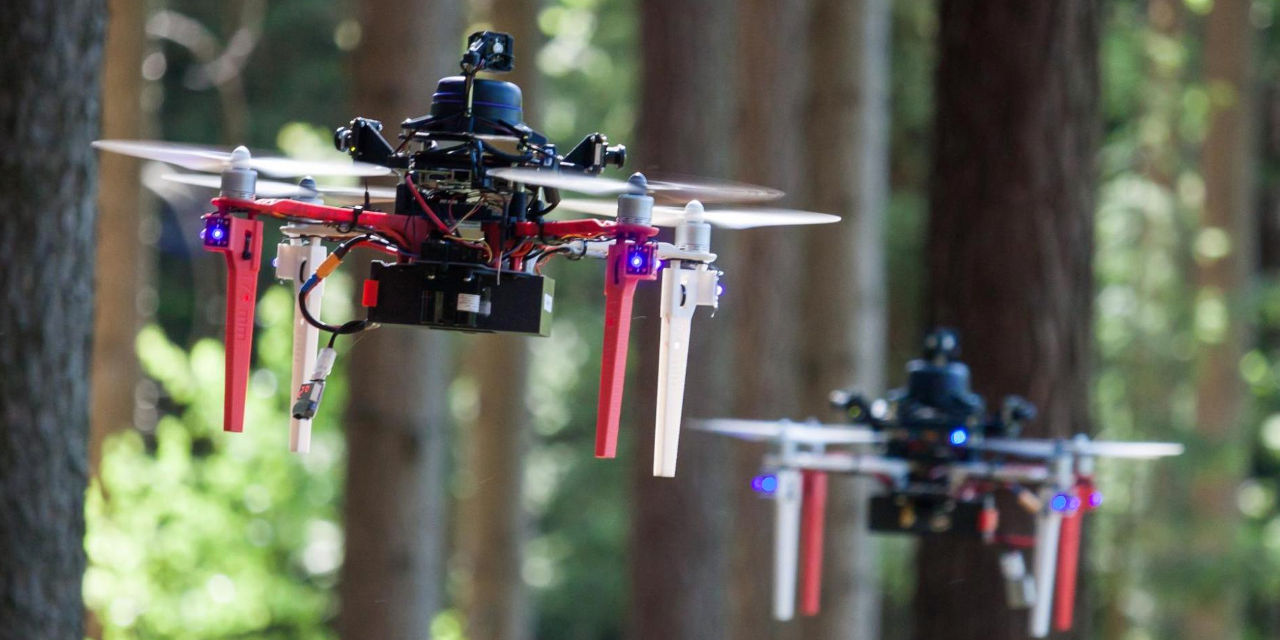
\includegraphics[height=10em]{./fig/photos/uvdar.jpg}};
    \begin{scope}[x={(a.south east)},y={(a.north west)}]
      %%{ grid
      % % useful grid to help you find coordinates for plotting the overlay
      % \draw[black, xstep=.1, ystep=.1] (0,0) grid (1,1);
      % \foreach \i in {0,0.1,0.2,0.3,0.4,0.5,0.6,0.7,0.8,0.9,1} {
      %   \node[align=center] at (\i, -0.05) {\i};
      %   \node[align=center] at (\i, 1.05) {\i};
      %   \node[align=center] at (-0.05, \i) {\i};
      %   \node[align=center] at (1.05, \i) {\i};
      % }
      %%}

      \draw[->, white, thick] (0.40, 0.20) -- (0.18, 0.59);
      \draw[->, white, thick] (0.40, 0.20) -- (0.48, 0.56);
      \draw[->, white, thick] (0.40, 0.20) -- (0.58, 0.24);
      \draw (0.40,0.15) node [text=white] {\small UV blinkers};

      \draw[->, white, thick] (0.80, 0.80) -- (0.80, 0.4);
      \draw[->, white, thick] (0.80, 0.80) -- (0.66, 0.4);
      \draw[->, white, thick] (0.80, 0.80) -- (0.50, 0.77);
      \draw (0.80,0.86) node [text=white] {\small UV cameras};

      % plot some stuff over the image
      \fill[white] (0.001, 0.001) rectangle (0.08,0.13);
      \fill[draw=black, draw opacity=0.5, fill opacity=0] (0,0) rectangle (1, 1);

      \node[imgletter,text=black] (label) at (a.south west) {(a)};
    \end{scope}
  \end{tikzpicture}}
  \hfill%
  \subfloat {\begin{tikzpicture}
    \node[anchor=south west,inner sep=0] (a) at (0,0) { 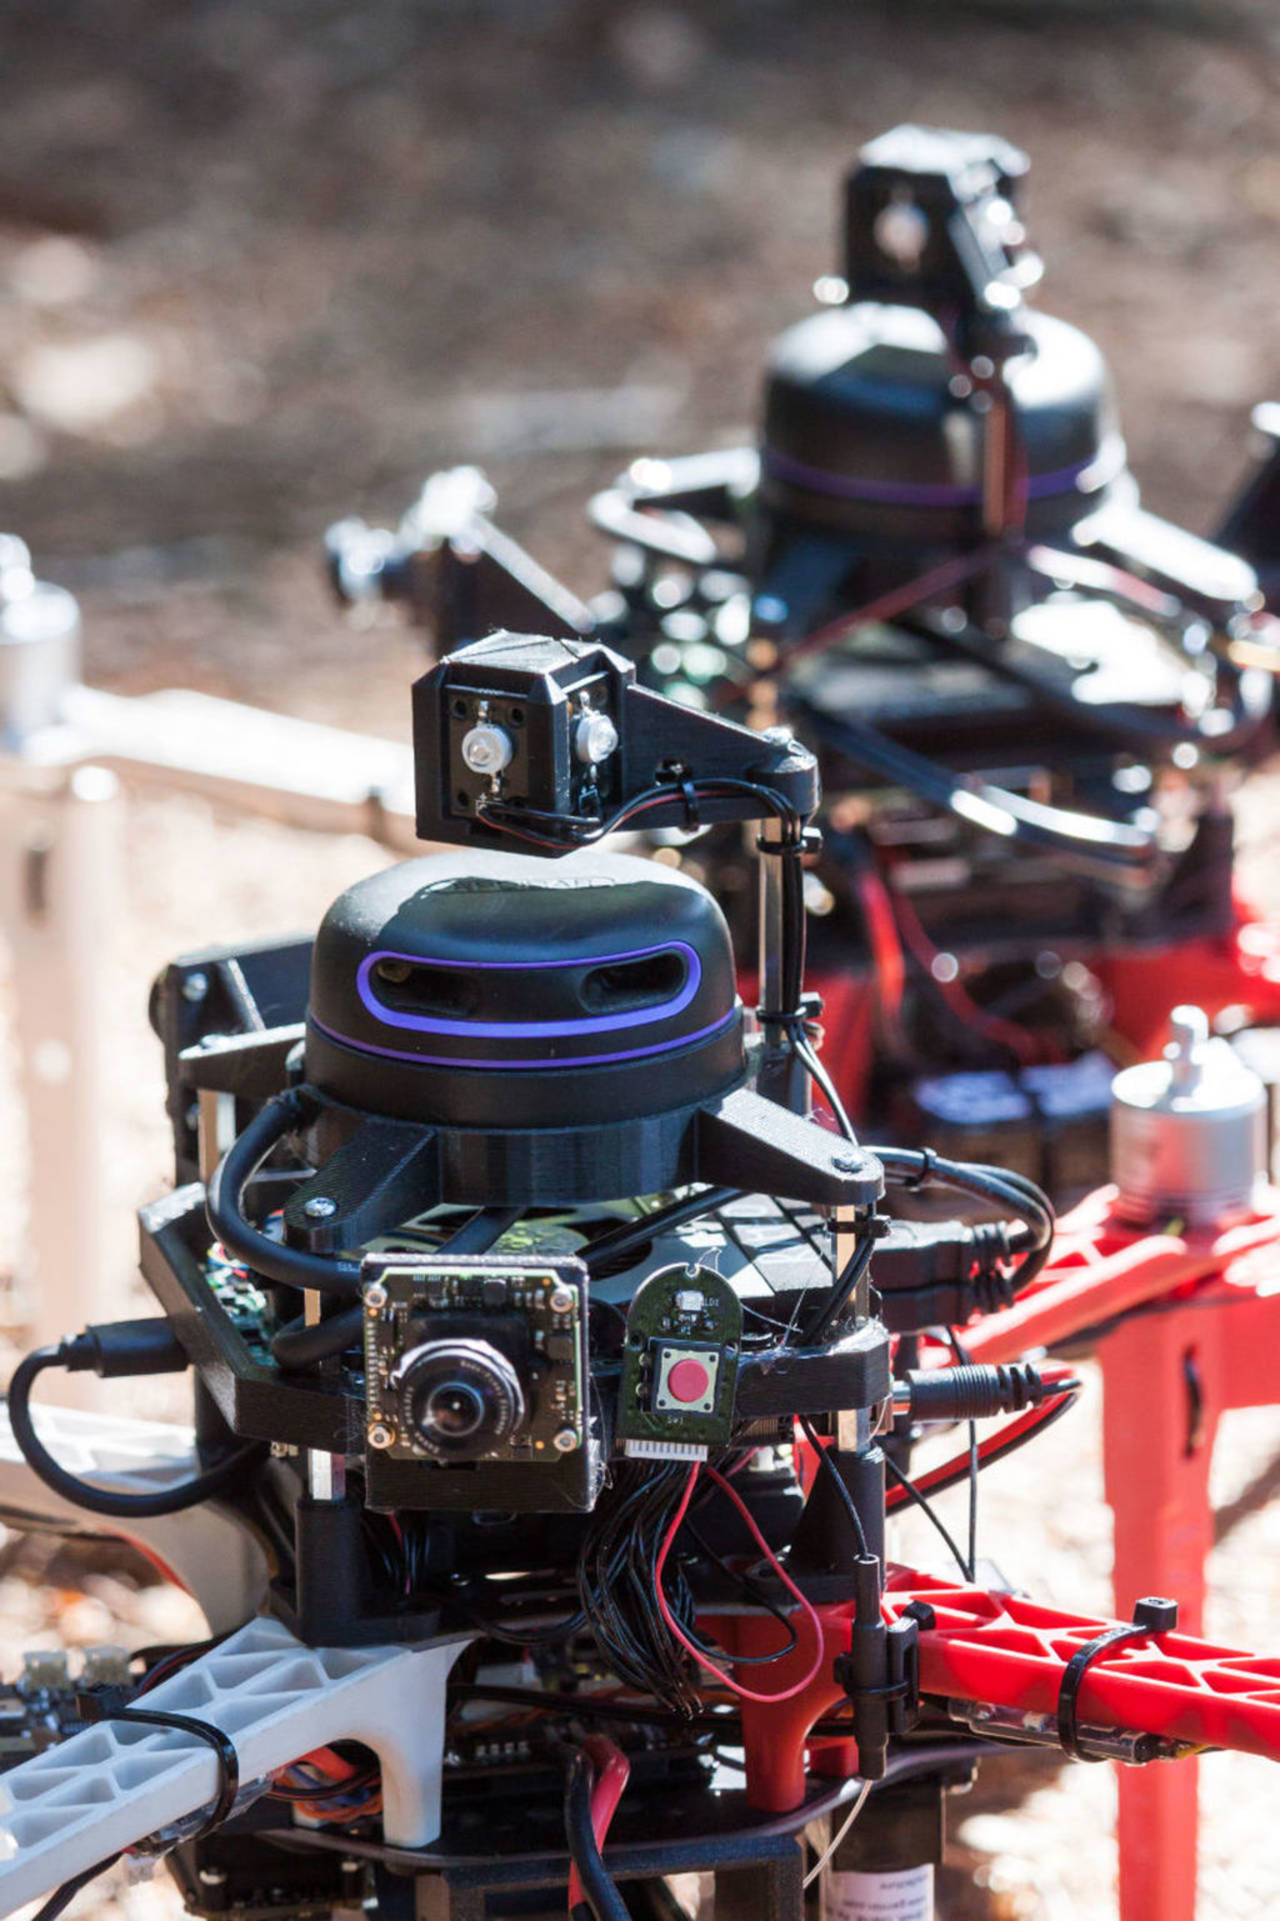
\includegraphics[height=10em]{./fig/photos/uvdar_camera.jpg}};
    \begin{scope}[x={(a.south east)},y={(a.north west)}]
      %%{ grid
      % % useful grid to help you find coordinates for plotting the overlay
      % \draw[black, xstep=.1, ystep=.1] (0,0) grid (1,1);
      % \foreach \i in {0,0.1,0.2,0.3,0.4,0.5,0.6,0.7,0.8,0.9,1} {
      %   \node[align=center] at (\i, -0.05) {\i};
      %   \node[align=center] at (\i, 1.05) {\i};
      %   \node[align=center] at (-0.05, \i) {\i};
      %   \node[align=center] at (1.05, \i) {\i};
      % }
      %%}
      % plot some stuff over the image
      \fill[white] (0.001, 0.001) rectangle (0.20,0.13);
      \fill[draw=black, draw opacity=0.5, fill opacity=0] (0,0) rectangle (1, 1);

      \node[imgletter,text=black] (label) at (a.south west) {(b)};
    \end{scope}
  \end{tikzpicture}}
  \caption{Mutual localization of \acp{UAV} by the UVDAR system is provided by (a) \ac{UV} blinkers on the \ac{UAV} arms and top. The blinkers are observed by onboard cameras (b) equipped with \ac{UV} band pass filters.}
  \label{fig:uvdar}
\end{figure}

%%}

%%{ Sub: Motion planning

\subsection{UAV motion planning}

Basic research on optimal planning for data collection with \acp{UAV} was studied in \cite{penicka2019data, penicka2017dubins, penicka2017neighborhoods, penicka2017reactive, faigl2017onsolution}.

\fullciteinbox{faigl2017onsolution}{}

The platform provided real-world verification and showed the feasibility of the proposed approaches.
Coverage optimization for multi-\ac{UAV} cooperative surveillance was tackled in \cite{petrlik2019coverage, faigl2019unsupervised}.
Complex maneuvers and cooperative load-carrying by multiple \acp{UAV} were reported on in \cite{spurny2019transport}.

\fullciteinbox{spurny2016complex}{}

%%}

%%{ Sub: Automatic control

\subsection{Automatic control}

A system for automatic gain tuning for the \emph{geometric tracking controller on SE(3)} was published in \cite{giernacki2019realtime}.

\fullciteinbox{giernacki2019realtime}{}

A novel optimal control design approach for automatic fire extinguishing is showcased in \cite{saikin2020wildfire}.

\fullciteinbox{saikin2020wildfire}{}

The properties of the SE(3) geometric feedback proved crucial for verifying the feasibility of the almost-free-fall trajectories designed to dispatch water during extreme maneuvers (see \reffig{fig:control}).

%%{ Fig: generic control and eagle

\begin{figure}
  \centering
  \subfloat {\begin{tikzpicture}
    \node[anchor=south west,inner sep=0] (a) at (0,0) { 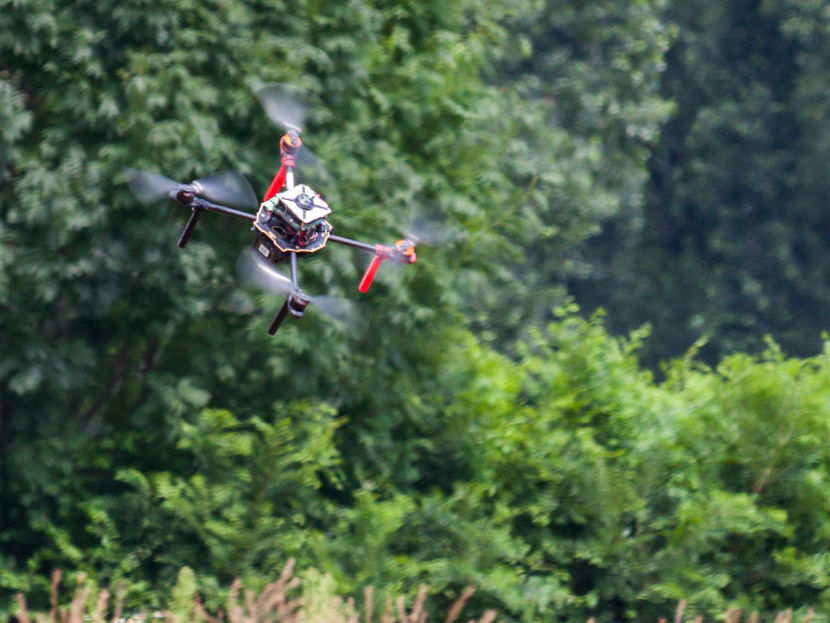
\includegraphics[width=0.235\textwidth]{./fig/photos/control_2_1-5.jpg}};
    \begin{scope}[x={(a.south east)},y={(a.north west)}]
      %%{ grid
      % % useful grid to help you find coordinates for plotting the overlay
      % \draw[black, xstep=.1, ystep=.1] (0,0) grid (1,1);
      % \foreach \i in {0,0.1,0.2,0.3,0.4,0.5,0.6,0.7,0.8,0.9,1} {
      %   \node[align=center] at (\i, -0.05) {\i};
      %   \node[align=center] at (\i, 1.05) {\i};
      %   \node[align=center] at (-0.05, \i) {\i};
      %   \node[align=center] at (1.05, \i) {\i};
      % }
      %%}
      % plot some stuff over the image
      \fill[white] (0.001, 0.001) rectangle (0.12,0.13);
      \fill[draw=black, draw opacity=0.5, fill opacity=0] (0,0) rectangle (1, 1);
      \node[imgletter,text=black] (label) at (a.south west) {(a)};
    \end{scope}
  \end{tikzpicture}}
  \hfill%
  \subfloat {\begin{tikzpicture}
    \node[anchor=south west,inner sep=0] (a) at (0,0) { 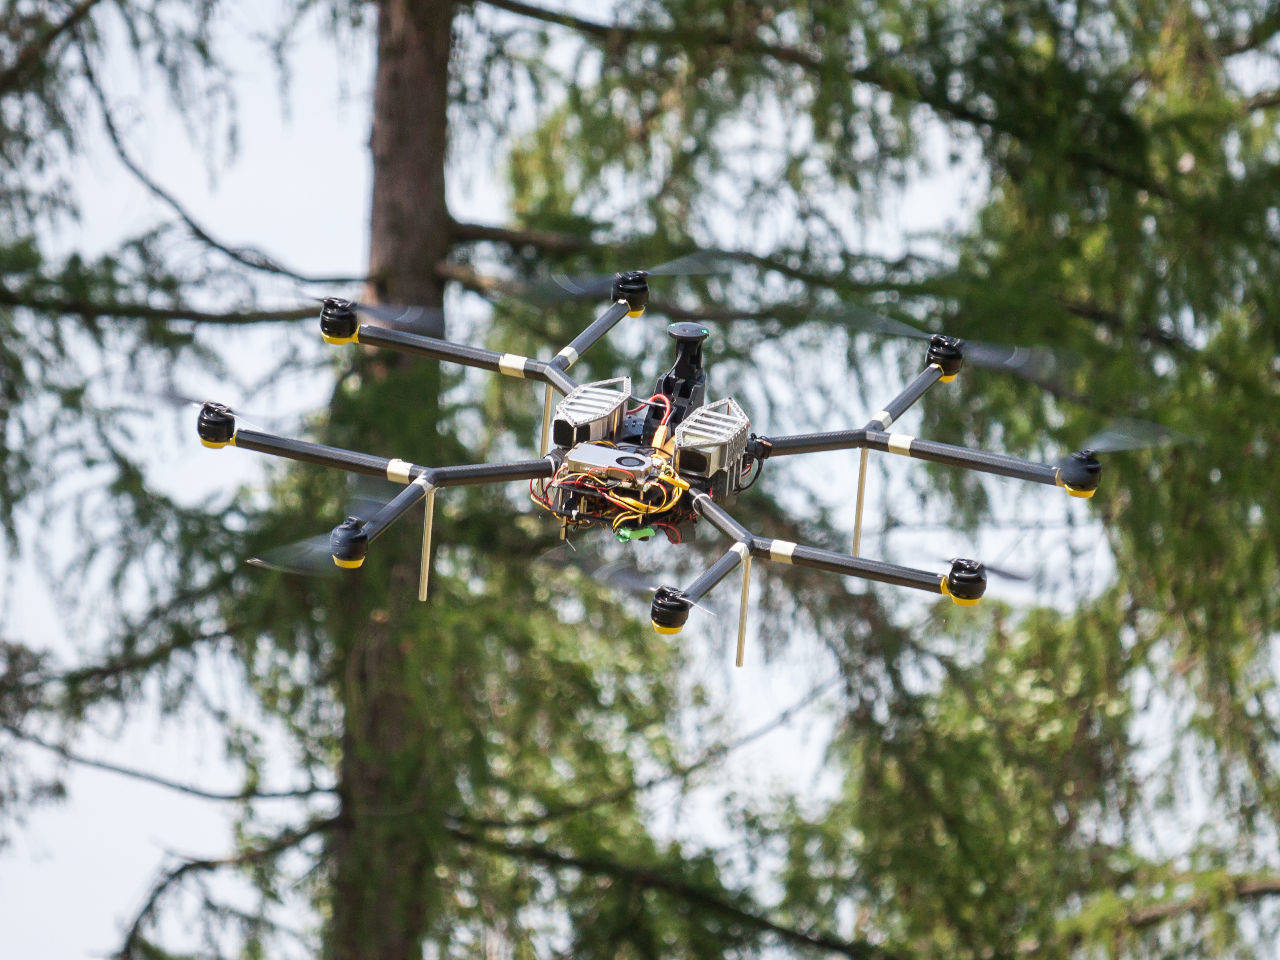
\includegraphics[width=0.235\textwidth]{./fig/photos/eagle_2_1-5.jpg}};
    \begin{scope}[x={(a.south east)},y={(a.north west)}]
      %%{ grid
      % % useful grid to help you find coordinates for plotting the overlay
      % \draw[black, xstep=.1, ystep=.1] (0,0) grid (1,1);
      % \foreach \i in {0,0.1,0.2,0.3,0.4,0.5,0.6,0.7,0.8,0.9,1} {
      %   \node[align=center] at (\i, -0.05) {\i};
      %   \node[align=center] at (\i, 1.05) {\i};
      %   \node[align=center] at (-0.05, \i) {\i};
      %   \node[align=center] at (1.05, \i) {\i};
      % }
      %%}
      % plot some stuff over the image
      \fill[white] (0.001, 0.001) rectangle (0.12,0.13);
      \fill[draw=black, draw opacity=0.5, fill opacity=0] (0,0) rectangle (1, 1);
      \node[imgletter,text=black] (label) at (a.south west) {(b)};
    \end{scope}
  \end{tikzpicture}}
  \caption{Novel control approaches can be tested on a real hardware. Off-the-shelf platforms such as (a) Tarot 650, and also (b) custom-built airframes, can be equipped with the proposed system.}
  \label{fig:control}
\end{figure}

%%}

%%}

\subsection{Data gathering}

\fullciteinbox{saska2017documentation}{}
The system is being used actively in a project working on indoor aerial inspection of historical buildings and monuments \cite{petracek2020dronument, kratky2020autonomous}.
Within this scenario, a \ac{UAV} is equipped with a 3D \ac{LiDAR} sensor and is automatically guided through an indoor environment, where it captures detailed imagery of hard-to-reach points of interest (see \reffig{fig:dronument}).
Similarly, transmission radio sources were automatically localized in \cite{vrba2019realtime}.

%%{ Fig: dronument

\begin{figure}
  \centering
  \subfloat {\begin{tikzpicture}
    \node[anchor=south west,inner sep=0] (a) at (0,0) { 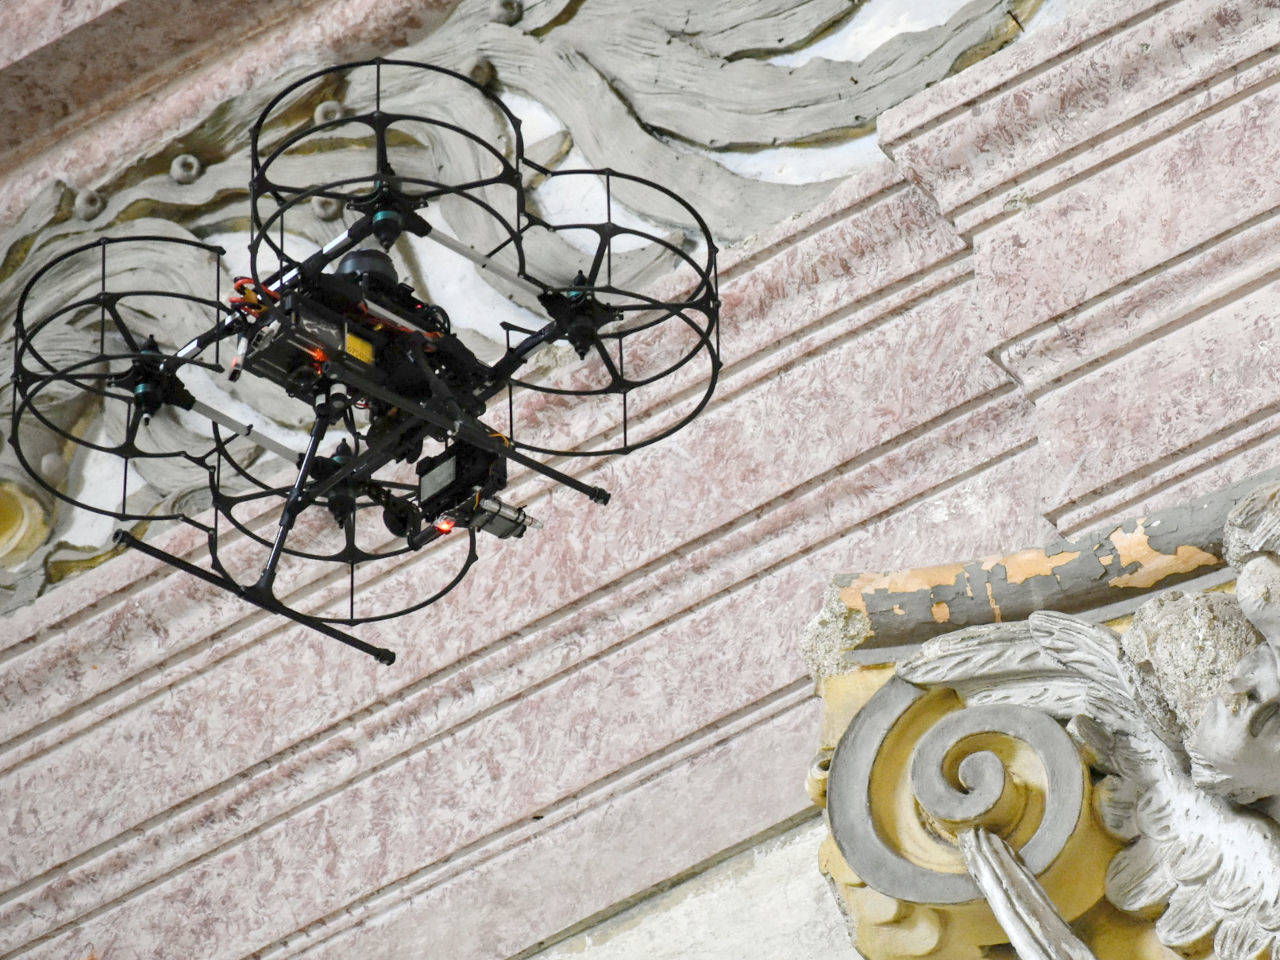
\includegraphics[width=0.235\textwidth]{./fig/photos/dronument_2_2_1-5.jpg}};
    \begin{scope}[x={(a.south east)},y={(a.north west)}]
      %%{ grid
      % % useful grid to help you find coordinates for plotting the overlay
      % \draw[black, xstep=.1, ystep=.1] (0,0) grid (1,1);
      % \foreach \i in {0,0.1,0.2,0.3,0.4,0.5,0.6,0.7,0.8,0.9,1} {
      %   \node[align=center] at (\i, -0.05) {\i};
      %   \node[align=center] at (\i, 1.05) {\i};
      %   \node[align=center] at (-0.05, \i) {\i};
      %   \node[align=center] at (1.05, \i) {\i};
      % }
      %%}
      % plot some stuff over the image
      \fill[white] (0.001, 0.001) rectangle (0.12,0.13);
      \fill[draw=black, draw opacity=0.5, fill opacity=0] (0,0) rectangle (1, 1);
      \node[imgletter,text=black] (label) at (a.south west) {(a)};
    \end{scope}
  \end{tikzpicture}}
  \hfill%
  \subfloat {\begin{tikzpicture}
    \node[anchor=south west,inner sep=0] (a) at (0,0) { 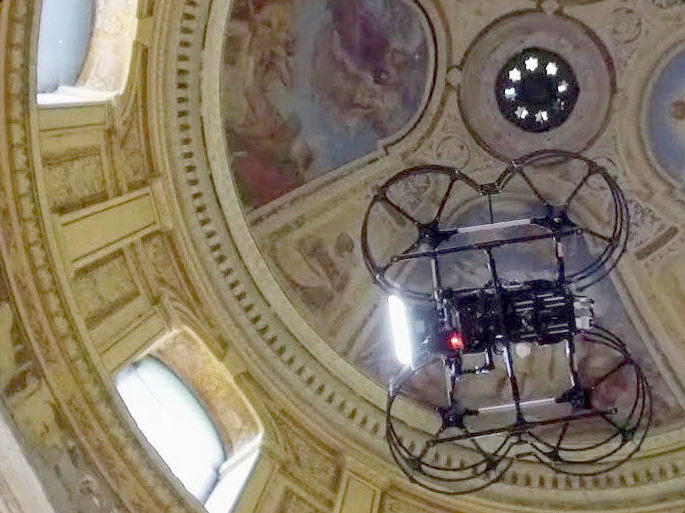
\includegraphics[width=0.235\textwidth]{./fig/photos/dronument_2_1-5.jpg}};
    \begin{scope}[x={(a.south east)},y={(a.north west)}]
      %%{ grid
      % % useful grid to help you find coordinates for plotting the overlay
      % \draw[black, xstep=.1, ystep=.1] (0,0) grid (1,1);
      % \foreach \i in {0,0.1,0.2,0.3,0.4,0.5,0.6,0.7,0.8,0.9,1} {
      %   \node[align=center] at (\i, -0.05) {\i};
      %   \node[align=center] at (\i, 1.05) {\i};
      %   \node[align=center] at (-0.05, \i) {\i};
      %   \node[align=center] at (1.05, \i) {\i};
      % }
      %%}
      % plot some stuff over the image
      \fill[white] (0.001, 0.001) rectangle (0.12,0.13);
      \fill[draw=black, draw opacity=0.5, fill opacity=0] (0,0) rectangle (1, 1);
      \node[imgletter,text=black] (label) at (a.south west) {(b)};
    \end{scope}
  \end{tikzpicture}}
  \caption{An inspection of an indoor historical building is conducted (a) to monitor the state of frescoes, and (b) to assess the state of wall paintings.}
  \label{fig:dronument}
\end{figure}

%%}

\subsection{UAV swarms and formations}
\label{sec:uav_swarms_and_formations}

Basic research in the area of \ac{UAV} swarming and formation flying was studied in \cite{saska2020formation, saska2016formations, saska2019large}.
\ac{UAV} swarm control is a relatively new field of research, and its applications are yet to be explored.
One of many possibilities being explored by the authors is the use of \acp{UAV} for inspecting hard-to-access locations such as power line towers without putting personnel at risk\footnote{\url{https://aerial-core.eu}}.
% The need for a swarm of \acp{UAV} is essential in this type of application.
This type of application requires the swarm coordination to be flexible, and to move, while minimizing the observed object estimation error.
% A crucial piece of information required for coordination of multi-robot systems working in the same workspace is a precise knowledge of mutual states of teammates.
Flocking capabilities are being explored within the framework of ongoing projects with real-world experiments in a field, and also within a forest environment (see \reffig{fig:swarms}).
Interactions between \acp{UAV} are studied in order to overcome challenging situations such as GNSS-denied environment navigation.

%%{ Fig: swamrs

\begin{figure}
  \centering
  \subfloat {\begin{tikzpicture}
    \node[anchor=south west,inner sep=0] (a) at (0,0) { 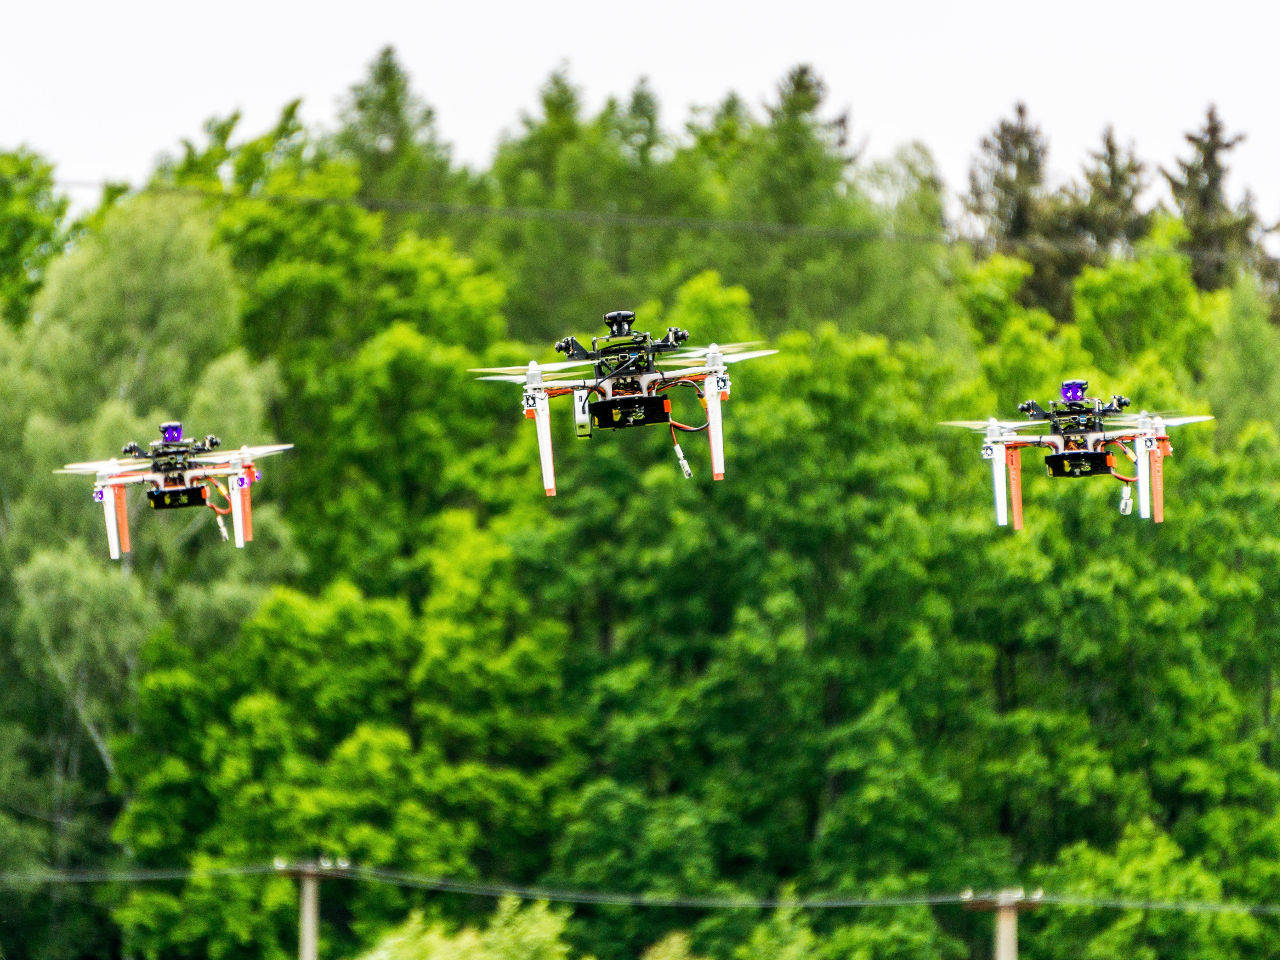
\includegraphics[width=0.235\textwidth]{./fig/photos/swarm_2_1-5.jpg}};
    \begin{scope}[x={(a.south east)},y={(a.north west)}]
      %%{ grid
      % % useful grid to help you find coordinates for plotting the overlay
      % \draw[black, xstep=.1, ystep=.1] (0,0) grid (1,1);
      % \foreach \i in {0,0.1,0.2,0.3,0.4,0.5,0.6,0.7,0.8,0.9,1} {
      %   \node[align=center] at (\i, -0.05) {\i};
      %   \node[align=center] at (\i, 1.05) {\i};
      %   \node[align=center] at (-0.05, \i) {\i};
      %   \node[align=center] at (1.05, \i) {\i};
      % }
      %%}
      \fill[white] (0.001, 0.001) rectangle (0.12,0.13);
      % plot some stuff over the image
      \fill[draw=black, draw opacity=0.5, fill opacity=0] (0,0) rectangle (1, 1);
      \node[imgletter,text=black] (label) at (a.south west) {(a)};
    \end{scope}
  \end{tikzpicture}}
  \hfill
  \subfloat {\begin{tikzpicture}
    \node[anchor=south west,inner sep=0] (a) at (0,0) { 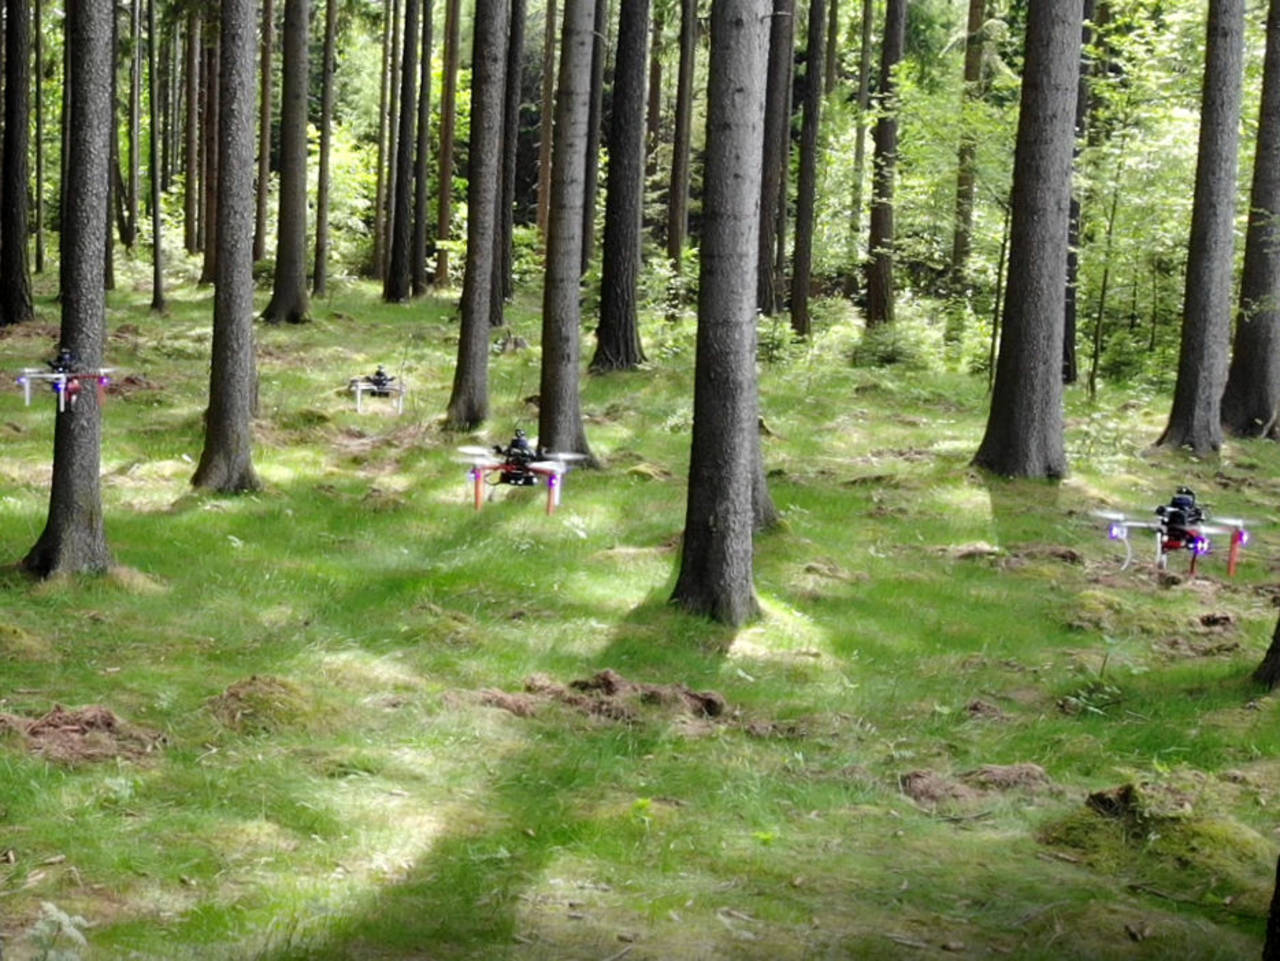
\includegraphics[width=0.235\textwidth]{./fig/photos/swarm_forest_2_1-5.jpg}};
    \begin{scope}[x={(a.south east)},y={(a.north west)}]
      %%{ grid
      % useful grid to help you find coordinates for plotting the overlay
      % \draw[black, xstep=.1, ystep=.1] (0,0) grid (1,1);
      % \foreach \i in {0,0.1,0.2,0.3,0.4,0.5,0.6,0.7,0.8,0.9,1} {
      %   \node[align=center] at (\i, -0.05) {\i};
      %   \node[align=center] at (\i, 1.05) {\i};
      %   \node[align=center] at (-0.05, \i) {\i};
      %   \node[align=center] at (1.05, \i) {\i};
      % }
      %%}

      \draw[->, white, thick] (0.45, 0.20) -- (0.07, 0.57);
      \draw[->, white, thick] (0.45, 0.20) -- (0.30, 0.55);
      \draw[->, white, thick] (0.45, 0.20) -- (0.40, 0.45);
      \draw[->, white, thick] (0.45, 0.20) -- (0.85, 0.40);
      \draw (0.45,0.15) node [text=white] {\small UAVs};

      \fill[white] (0.001, 0.001) rectangle (0.12,0.13);
      % plot some stuff over the image
      \fill[draw=black, draw opacity=0.5, fill opacity=0] (0,0) rectangle (1, 1);
      \node[imgletter,text=black] (label) at (a.south west) {(b)};
    \end{scope}
  \end{tikzpicture}}
  \caption{Swarms of multirotor \acp{UAV} testing novel flocking algorithms while localized (a) by a \ac{GNSS} system, and (b) by onboard sensors only within a forest environment.}
  \label{fig:swarms}
\end{figure}

%%}

% Most cited approaches, although achieving great results, lack reliability in terms of independence to changing environmental conditions in the real-world, which is not acceptable in such the proposed safety-critical work. This means that a fully distributed control approach is needed. To achieve that, we plan to apply our achievements in the endeavor to design a robust system usable in various environments, both relying on vision-based precise mutual object detection in UAV proximity \cite{krajnik14jint} as well as using robust active UV patterns to solve this problem \cite{Walter2018}.

\subsection{MBZIRC 2017 competition}

The \ac{MBZIRC} 2017\footnote{MBZIRC 2017, \url{http://mbzirc.com/challenge/2017}} aimed at pushing the frontiers of field robotics.
Two tasks out of the three challenges within the competition were focused solely on aerial manipulation and UAV control.
The competition imposed real-world constraints in its tasks that forced the participating teams to show the current state of the art in robotics and to perform the tasks within a short time window and within specified time slots.
The first task --- autonomous gathering of colored ferrous objects by a group of \acp{UAV} --- was successfully tackled by the CTU-UPENN-UoL\footnote{Collaboration of Czech Technical University in Prague, University of Pennsylvania, and the University of Lincoln.} team, using the proposed system \cite{spurny2019cooperative, faigl2019unsupervised, loianno2018localization} (see \reffig{fig:mbzirc_2017}).
We won 1$^{\mathrm{st}}$ place among the best teams from all over the world.
The second task of autonomous landing on a moving car was also tackled by the proposed system.
We achieved the fastest autonomous landing among all the teams, and we took the 2$^{\text{nd}}$ place overall in the competition \cite{baca2019autonomous, stepan2019vision}.

%%{ Fig: MBZIRC 2017

\begin{figure}
  \centering
  \subfloat {\begin{tikzpicture}
    \node[anchor=south west,inner sep=0] (a) at (0,0) { 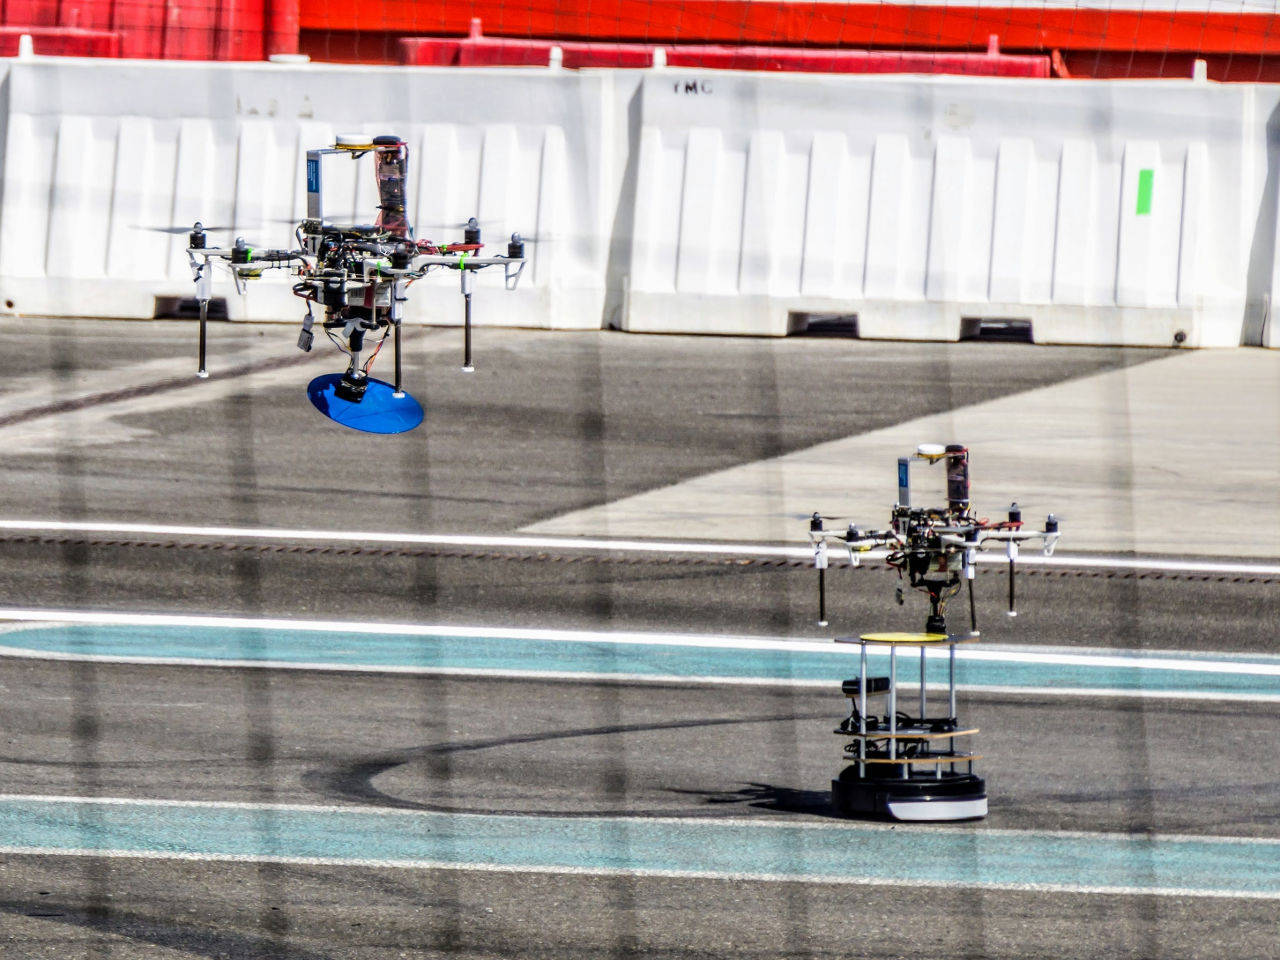
\includegraphics[width=0.235\textwidth]{./fig/photos/grasping_2017_2_1-5.jpg}};
    \begin{scope}[x={(a.south east)},y={(a.north west)}]
      %%{ grid
      % % useful grid to help you find coordinates for plotting the overlay
      % \draw[black, xstep=.1, ystep=.1] (0,0) grid (1,1);
      % \foreach \i in {0,0.1,0.2,0.3,0.4,0.5,0.6,0.7,0.8,0.9,1} {
      %   \node[align=center] at (\i, -0.05) {\i};
      %   \node[align=center] at (\i, 1.05) {\i};
      %   \node[align=center] at (-0.05, \i) {\i};
      %   \node[align=center] at (1.05, \i) {\i};
      % }
      %%}
      % plot some stuff over the image
      \fill[white] (0.001, 0.001) rectangle (0.12,0.13);
      \fill[draw=black, draw opacity=0.5, fill opacity=0] (0,0) rectangle (1, 1);
      \node[imgletter,text=black] (label) at (a.south west) {(a)};
    \end{scope}
  \end{tikzpicture}}
  \hfill%
  \subfloat {\begin{tikzpicture}
    \node[anchor=south west,inner sep=0] (a) at (0,0) { 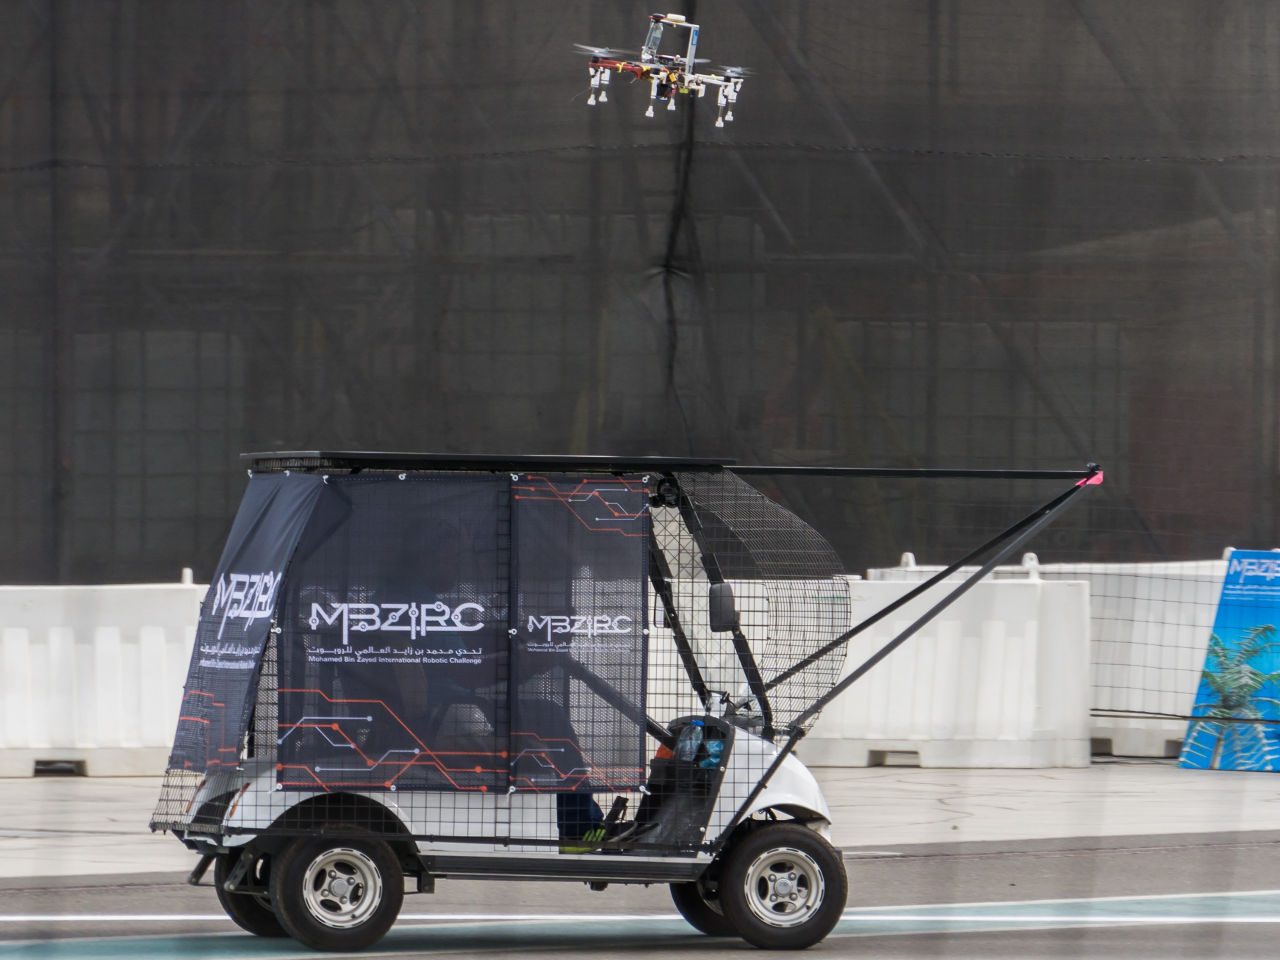
\includegraphics[width=0.235\textwidth]{./fig/photos/landing_2017_2_1-5.jpg}};
    \begin{scope}[x={(a.south east)},y={(a.north west)}]
      %%{ grid
      % % useful grid to help you find coordinates for plotting the overlay
      % \draw[black, xstep=.1, ystep=.1] (0,0) grid (1,1);
      % \foreach \i in {0,0.1,0.2,0.3,0.4,0.5,0.6,0.7,0.8,0.9,1} {
      %   \node[align=center] at (\i, -0.05) {\i};
      %   \node[align=center] at (\i, 1.05) {\i};
      %   \node[align=center] at (-0.05, \i) {\i};
      %   \node[align=center] at (1.05, \i) {\i};
      % }
      %%}
      % plot some stuff over the image
      \fill[white] (0.001, 0.001) rectangle (0.12,0.13);
      \fill[draw=black, draw opacity=0.5, fill opacity=0] (0,0) rectangle (1, 1);
      \node[imgletter,text=black] (label) at (a.south west) {(b)};
    \end{scope}
  \end{tikzpicture}}
  \caption{The CTU-UPENN-UoL team during the MBZIRC 2017 competition. The photos show (a) two \acp{UAV} while delivering ferrous objects, and (b) a \ac{UAV} during autonomous landing on a moving car.}
  \label{fig:mbzirc_2017}
\end{figure}

%%}

\subsection{The DARPA Subterranean (SubT) challenge}

The \ac{DARPA}, an agency of the United States Department of Defense, organizes series of challenges focused on automatic search \& rescue in an underground environment --- the \ac{DARPA} Subterranean challenge.
In the \ac{DARPA} Tunnel Circuit, the first round of the challenge, we deployed autonomous \acp{UAV} and semi-autonomous ground robots to explore underground mine shafts \cite{petrlik2020robust, roucek2019darpa}.
Our team deployed autonomous \acp{UAV} with the proposed system (see \reffig{fig:darpa}), which navigated the underground tunnels and returned safely to the entrance while autonomously localizing objects of interest.
We won the 1$^{\mathrm{st}}$ prize among the self-funded teams and the 3$^{\mathrm{rd}}$ prize overall.
To the best of our knowledge, our \acp{UAV} managed to explore a greater distance into the tunnels than any of the other teams.

%%{ Fig: DARPA SubT

\begin{figure}
  \centering
  \subfloat {\begin{tikzpicture}
    \node[anchor=south west,inner sep=0] (a) at (0,0) { 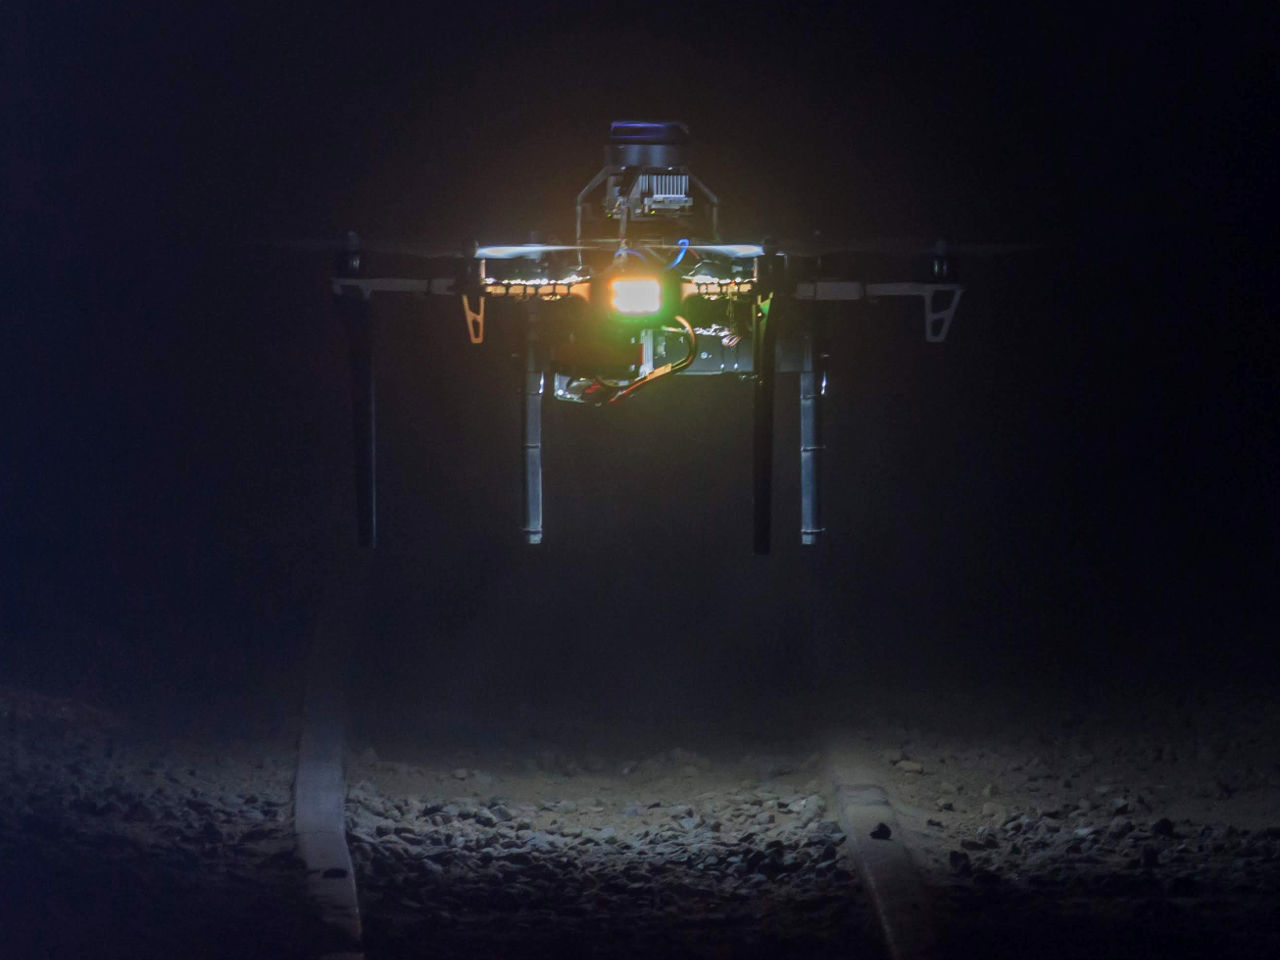
\includegraphics[width=0.235\textwidth]{./fig/photos/darpa_stix_2_1-5.jpg}};
    \begin{scope}[x={(a.south east)},y={(a.north west)}]
      %%{ grid
      % % useful grid to help you find coordinates for plotting the overlay
      % \draw[black, xstep=.1, ystep=.1] (0,0) grid (1,1);
      % \foreach \i in {0,0.1,0.2,0.3,0.4,0.5,0.6,0.7,0.8,0.9,1} {
      %   \node[align=center] at (\i, -0.05) {\i};
      %   \node[align=center] at (\i, 1.05) {\i};
      %   \node[align=center] at (-0.05, \i) {\i};
      %   \node[align=center] at (1.05, \i) {\i};
      % }
      %%}
      % plot some stuff over the image
      \fill[white] (0.001, 0.001) rectangle (0.12,0.13);
      \fill[draw=black, draw opacity=0.5, fill opacity=0] (0,0) rectangle (1, 1);
      \node[imgletter,text=black] (label) at (a.south west) {(a)};
    \end{scope}
  \end{tikzpicture}}
  \hfill%
  \subfloat {\begin{tikzpicture}
    \node[anchor=south west,inner sep=0] (a) at (0,0) { 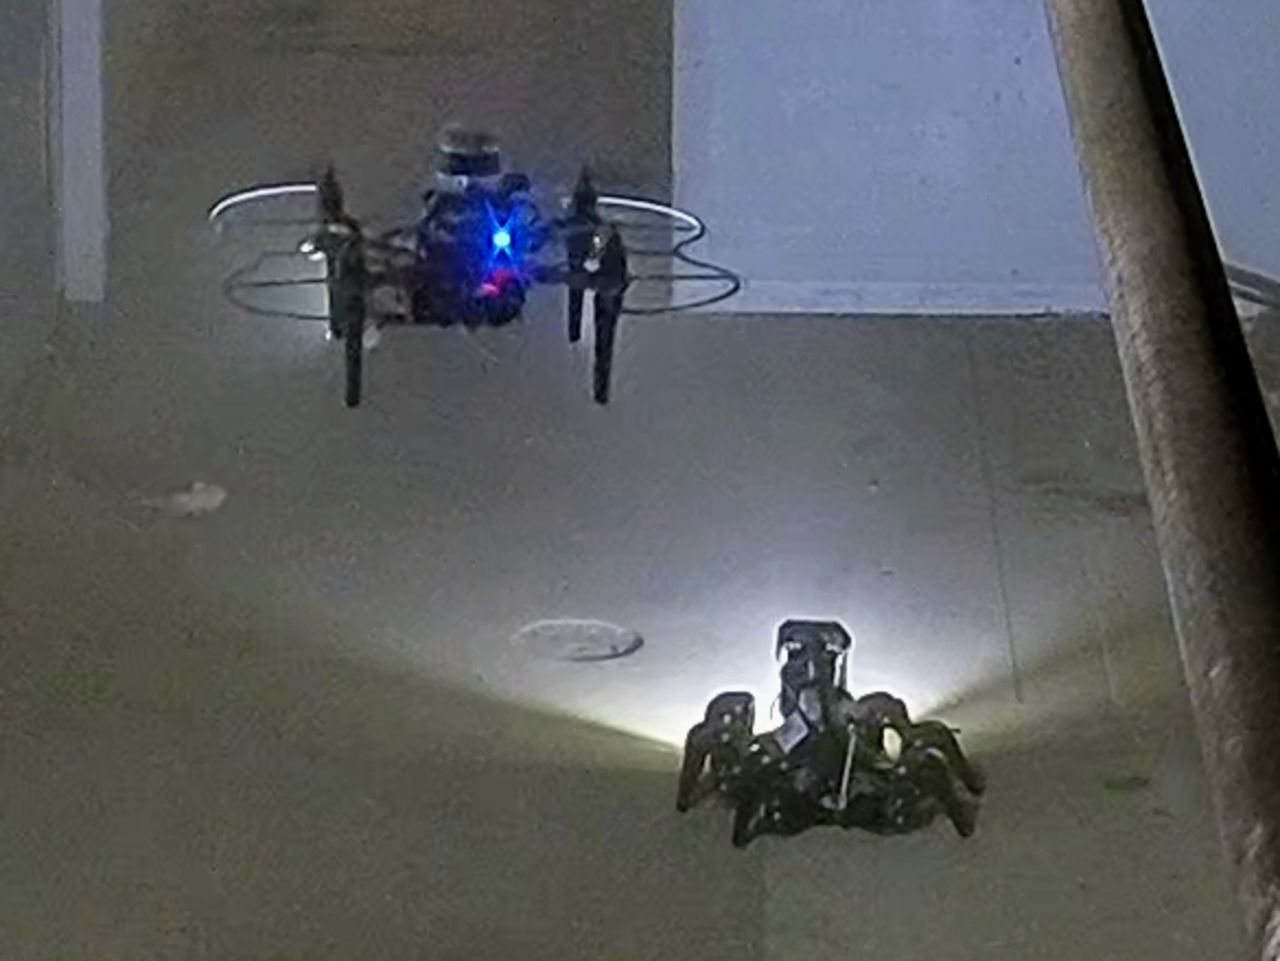
\includegraphics[width=0.235\textwidth]{./fig/photos/darpa_drone_beta_2_1-5.jpg}};
    \begin{scope}[x={(a.south east)},y={(a.north west)}]
      %%{ grid
      % % useful grid to help you find coordinates for plotting the overlay
      % \draw[black, xstep=.1, ystep=.1] (0,0) grid (1,1);
      % \foreach \i in {0,0.1,0.2,0.3,0.4,0.5,0.6,0.7,0.8,0.9,1} {
      %   \node[align=center] at (\i, -0.05) {\i};
      %   \node[align=center] at (\i, 1.05) {\i};
      %   \node[align=center] at (-0.05, \i) {\i};
      %   \node[align=center] at (1.05, \i) {\i};
      % }
      %%}
      % plot some stuff over the image
      \fill[white] (0.001, 0.001) rectangle (0.12,0.13);
      \fill[draw=black, draw opacity=0.5, fill opacity=0] (0,0) rectangle (1, 1);
      \node[imgletter,text=black] (label) at (a.south west) {(b)};
    \end{scope}
  \end{tikzpicture}}
  \caption{Unmanned Aerial Vehicles during the \ac{DARPA} SubT challenge. The photos depict (a) a \ac{UAV} exploring an underground mine, and (b) mapping an unfinished nuclear power plant.}
  \label{fig:darpa}
\end{figure}

%%}

In the \ac{DARPA} Urban Circuit, the second round of the challenge, we deployed autonomous \acp{UAV} and semi-autonomous ground robots to explore the infrastructure of an unfinished nuclear power plant.
Our \acp{UAV} managed to explore \SI{2867}{\meter\cubed} of one floor of the reactor building while automatically navigating up to \SI{100}{\meter} in just \SI{200}{\second} in a completely unknown environment.
We again took 1$^{\text{st}}$ place among the self-funded teams, and 3$^{\text{rd}}$ place overall.
Scientific publications on tasks within the Urban Circuit are under preparation.

\subsection{MBZIRC 2020 competition}

The second round of the \ac{MBZIRC} competition was organized in 2020.
It pushed the current state of the art in aerial robotics to its limits, with tasks such as organizing a group of \acp{UAV} and a \ac{UGV} to build a brick wall autonomously, autonomous indoor and outdoor firefighting with \acp{UAV}, and autonomously catching a ball carried by a \ac{UAV}, performed simultaneously with balloon popping by a group of \acp{UAV} (see \reffig{fig:mbzirc_2020}).
All of the tasks were solved using the proposed \ac{UAV} system, and our participation in the competition helped to consolidate many of the platform's functionalities.
The CTU-UPENN-NYU\footnote{Collaboration between the Czech Technical University in Prague, the University of Pennsylvania, and the New York University.} team achieved the highest score of all the teams for building the brick wall autonomously.
We also took $2^{\text{nd}}$ in the autonomous balloon popping and ball-catching task.
We won the gold medal in the \emph{grand challenge} in which all the tasks were tested simultaneously.
Scientific publications reporting on \ac{MBZIRC} 2020 are under preparation.

%%{ Fig: MBZIRC 2020

\begin{figure}
  \centering
  \subfloat {\begin{tikzpicture}
    \node[anchor=south west,inner sep=0] (a) at (0,0) { 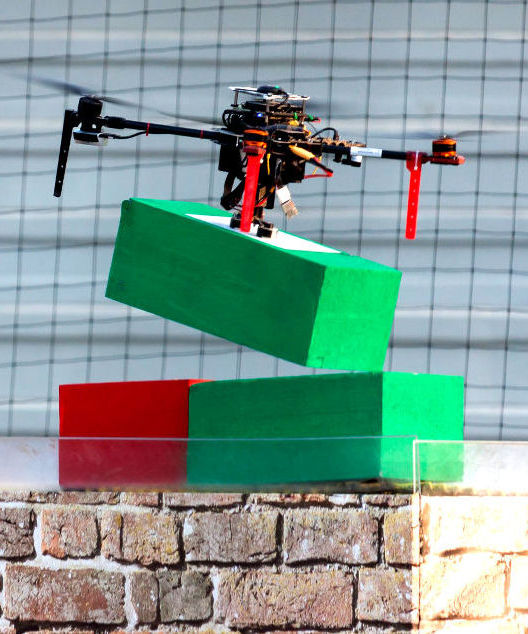
\includegraphics[width=0.155\textwidth]{./fig/photos/brick_placing_1-25_1-5.jpg}};
    \begin{scope}[x={(a.south east)},y={(a.north west)}]
      %%{ grid
      % % useful grid to help you find coordinates for plotting the overlay
      % \draw[black, xstep=.1, ystep=.1] (0,0) grid (1,1);
      % \foreach \i in {0,0.1,0.2,0.3,0.4,0.5,0.6,0.7,0.8,0.9,1} {
      %   \node[align=center] at (\i, -0.05) {\i};
      %   \node[align=center] at (\i, 1.05) {\i};
      %   \node[align=center] at (-0.05, \i) {\i};
      %   \node[align=center] at (1.05, \i) {\i};
      % }
      %%}
      % plot some stuff over the image
      \fill[white] (0.001, 0.001) rectangle (0.18,0.13);
      \fill[draw=black, draw opacity=0.5, fill opacity=0] (0,0) rectangle (1, 1);
      \node[imgletter,text=black] (label) at (a.south west) {(a)};
    \end{scope}
  \end{tikzpicture}}
  \hfill%
  \subfloat {\begin{tikzpicture}
    \node[anchor=south west,inner sep=0] (a) at (0,0) { 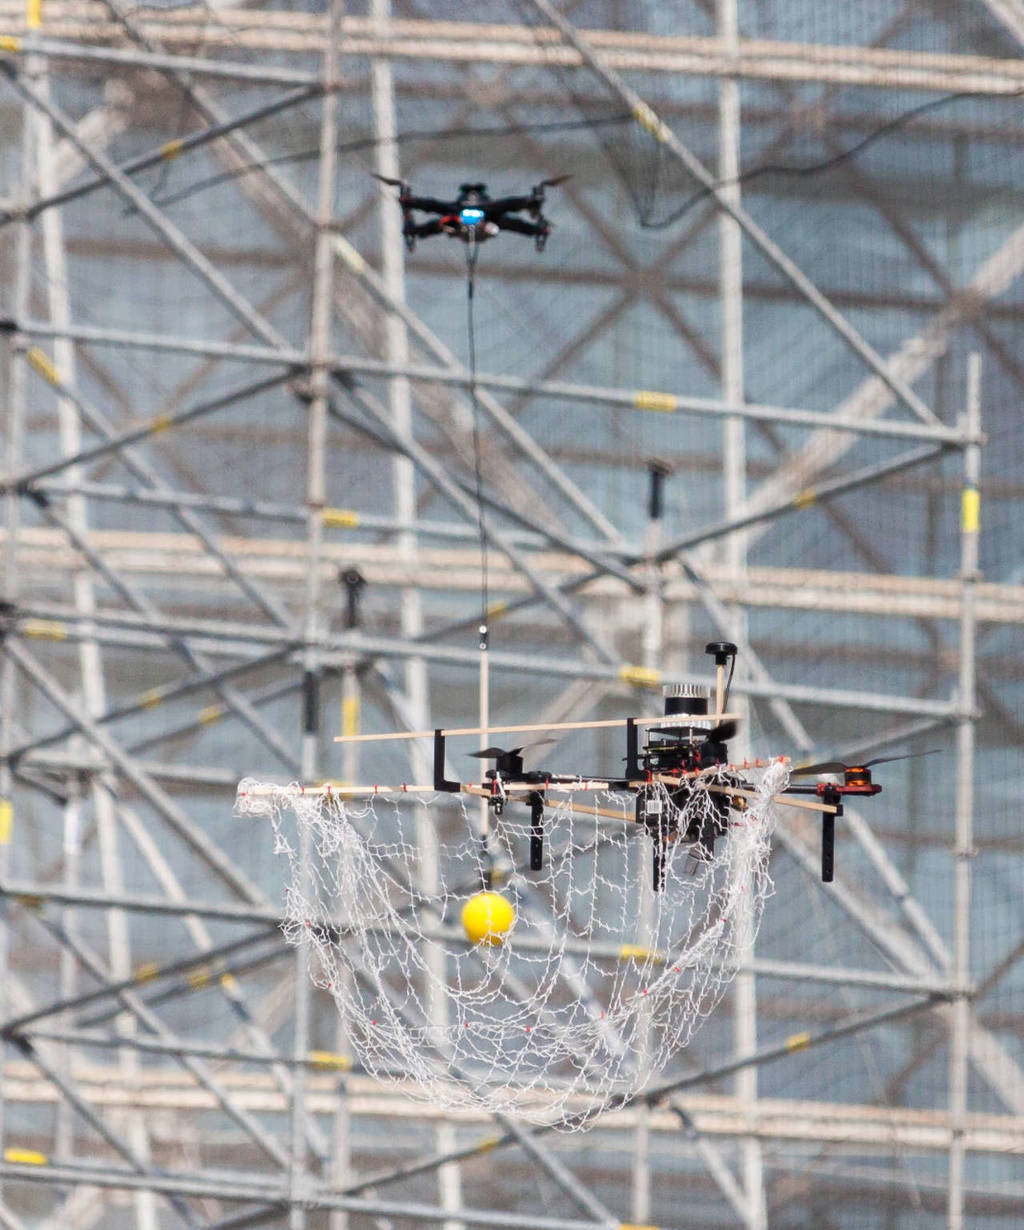
\includegraphics[width=0.155\textwidth]{./fig/photos/ball_catching_1-25_1-5.jpg}};
    \begin{scope}[x={(a.south east)},y={(a.north west)}]
      %%{ grid
      % % useful grid to help you find coordinates for plotting the overlay
      % \draw[black, xstep=.1, ystep=.1] (0,0) grid (1,1);
      % \foreach \i in {0,0.1,0.2,0.3,0.4,0.5,0.6,0.7,0.8,0.9,1} {
      %   \node[align=center] at (\i, -0.05) {\i};
      %   \node[align=center] at (\i, 1.05) {\i};
      %   \node[align=center] at (-0.05, \i) {\i};
      %   \node[align=center] at (1.05, \i) {\i};
      % }
      %%}
      % plot some stuff over the image
      \fill[white] (0.001, 0.001) rectangle (0.18,0.13);
      \fill[draw=black, draw opacity=0.5, fill opacity=0] (0,0) rectangle (1, 1);
      \node[imgletter,text=black] (label) at (a.south west) {(b)};
    \end{scope}
  \end{tikzpicture}}
  \hfill%
  \subfloat {\begin{tikzpicture}
    \node[anchor=south west,inner sep=0] (a) at (0,0) { 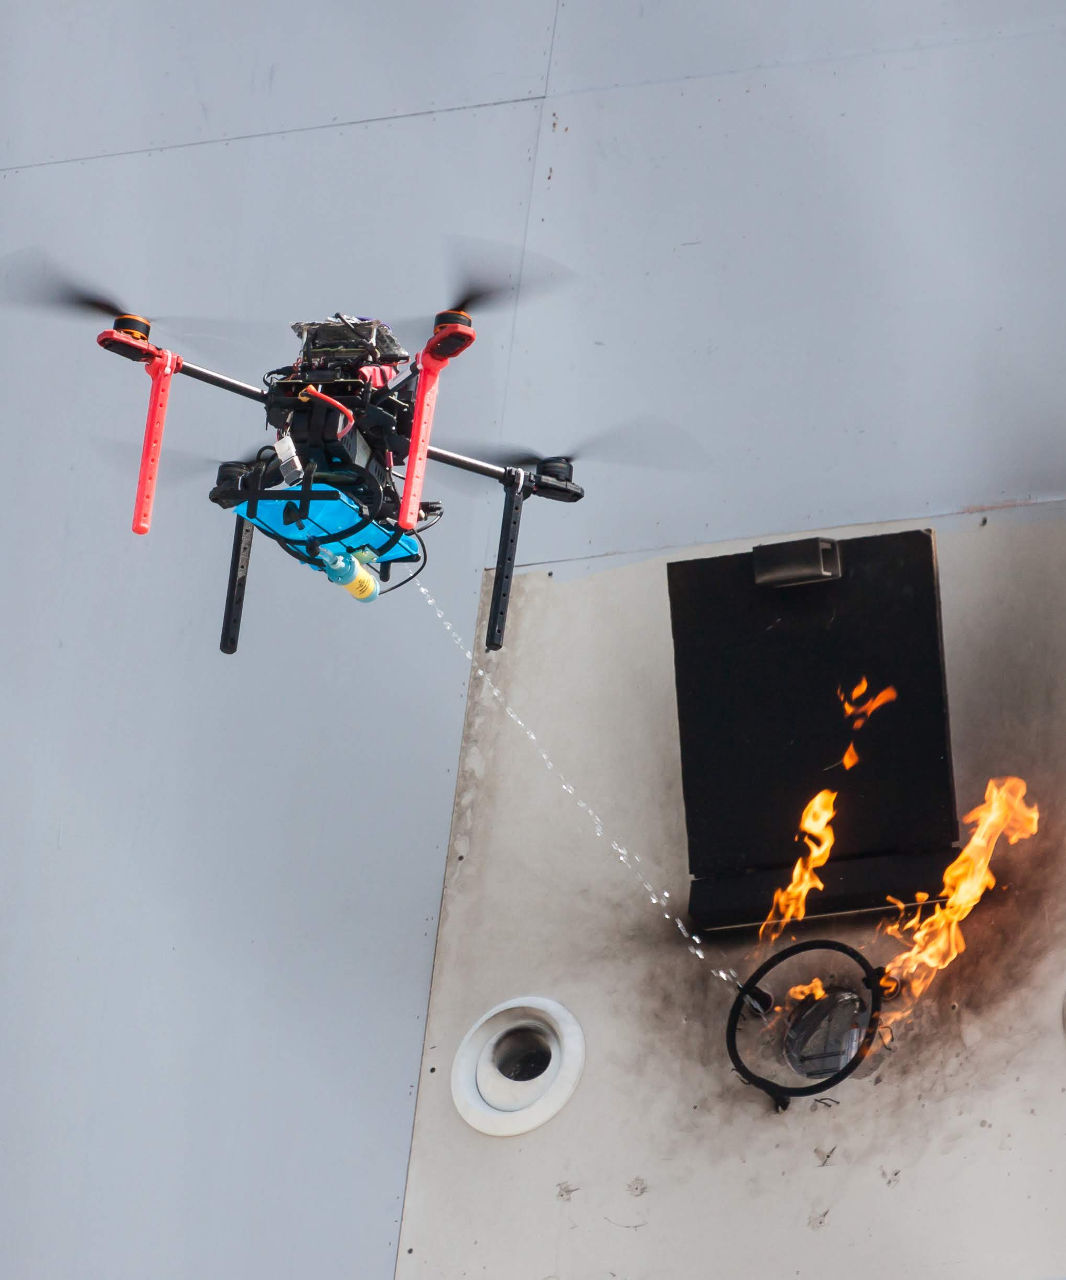
\includegraphics[width=0.155\textwidth]{./fig/photos/ext_1-25_1-5.jpg}};
    \begin{scope}[x={(a.south east)},y={(a.north west)}]
      %%{ grid
      % % useful grid to help you find coordinates for plotting the overlay
      % \draw[black, xstep=.1, ystep=.1] (0,0) grid (1,1);
      % \foreach \i in {0,0.1,0.2,0.3,0.4,0.5,0.6,0.7,0.8,0.9,1} {
      %   \node[align=center] at (\i, -0.05) {\i};
      %   \node[align=center] at (\i, 1.05) {\i};
      %   \node[align=center] at (-0.05, \i) {\i};
      %   \node[align=center] at (1.05, \i) {\i};
      % }
      %%}
      % plot some stuff over the image
      \fill[white] (0.001, 0.001) rectangle (0.18,0.13);
      \fill[draw=black, draw opacity=0.5, fill opacity=0] (0,0) rectangle (1, 1);
      \node[imgletter,text=black] (label) at (a.south west) {(c)};
    \end{scope}
  \end{tikzpicture}}\\
  \vspace{-0.8em}
  \subfloat {\begin{tikzpicture}
    \node[anchor=south west,inner sep=0] (a) at (0,0) { 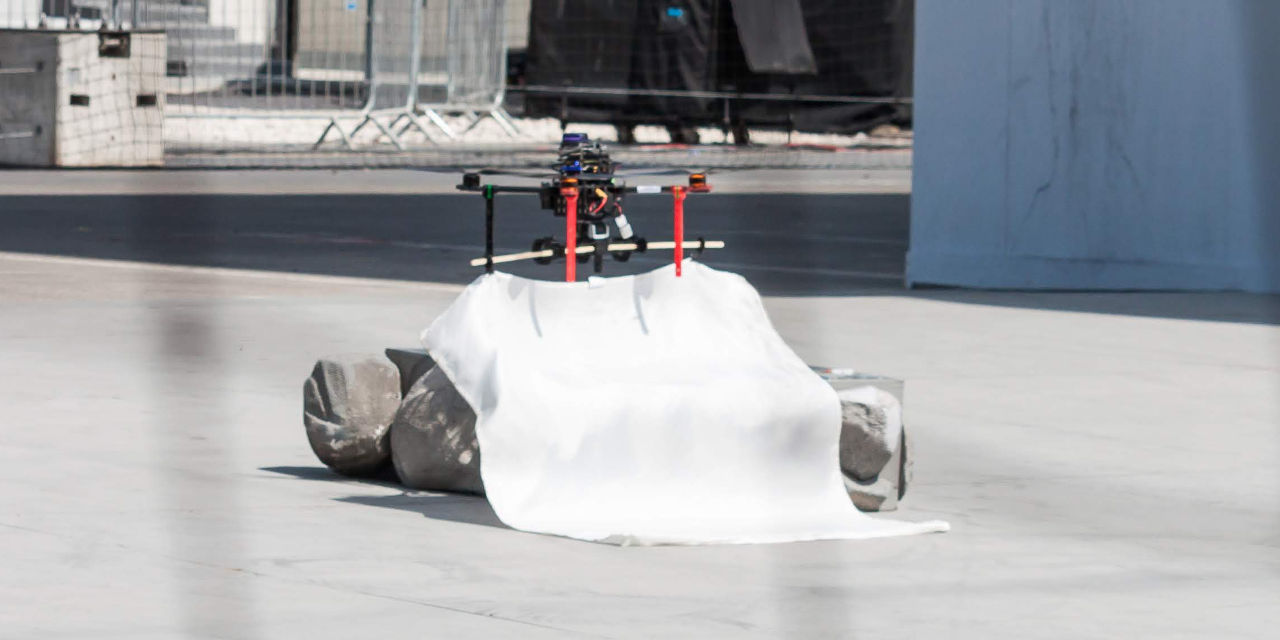
\includegraphics[width=0.235\textwidth]{./fig/photos/blanket_2_1.jpg}};
    \begin{scope}[x={(a.south east)},y={(a.north west)}]
      %%{ grid
      % % useful grid to help you find coordinates for plotting the overlay
      % \draw[black, xstep=.1, ystep=.1] (0,0) grid (1,1);
      % \foreach \i in {0,0.1,0.2,0.3,0.4,0.5,0.6,0.7,0.8,0.9,1} {
      %   \node[align=center] at (\i, -0.05) {\i};
      %   \node[align=center] at (\i, 1.05) {\i};
      %   \node[align=center] at (-0.05, \i) {\i};
      %   \node[align=center] at (1.05, \i) {\i};
      % }
      %%}
      % plot some stuff over the image
      \fill[white] (0.001, 0.001) rectangle (0.13,0.20);
      \fill[draw=black, draw opacity=0.5, fill opacity=0] (0,0) rectangle (1, 1);
      \node[imgletter,text=black] (label) at (a.south west) {(d)};
    \end{scope}
  \end{tikzpicture}}
  \hfill%
  \subfloat {\begin{tikzpicture}
    \node[anchor=south west,inner sep=0] (a) at (0,0) { 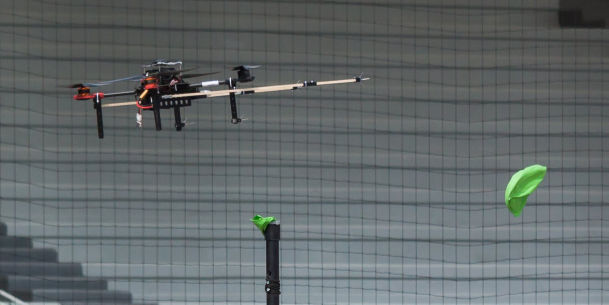
\includegraphics[width=0.235\textwidth]{./fig/photos/popping_2_1.jpg}};
    \begin{scope}[x={(a.south east)},y={(a.north west)}]
      %%{ grid
      % % useful grid to help you find coordinates for plotting the overlay
      % \draw[black, xstep=.1, ystep=.1] (0,0) grid (1,1);
      % \foreach \i in {0,0.1,0.2,0.3,0.4,0.5,0.6,0.7,0.8,0.9,1} {
      %   \node[align=center] at (\i, -0.05) {\i};
      %   \node[align=center] at (\i, 1.05) {\i};
      %   \node[align=center] at (-0.05, \i) {\i};
      %   \node[align=center] at (1.05, \i) {\i};
      % }
      %%}
      % plot some stuff over the image
      \fill[white] (0.001, 0.001) rectangle (0.13,0.20);
      \fill[draw=black, draw opacity=0.5, fill opacity=0] (0,0) rectangle (1, 1);
      \node[imgletter,text=black] (label) at (a.south west) {(e)};
    \end{scope}
  \end{tikzpicture}}
  \caption{The CTU-UPENN-NYU team during the MBZIRC 2020 competition. The photos depict (a) autonomous wall building, (b) autonomous ball catching, (c) autonomous fire extinguishing, (d) autonomous fire blanket deployment, and (e) autonomous balloon popping.}
  \label{fig:mbzirc_2020}
\end{figure}

%%}

\subsection{IEEE RAS Summer School on Multi-robot Systems}

The proposed system was used as an educational tool during the 2019 \ac{IEEE} \ac{RAS} summer school on multirobot systems\footnote{\url{http://mrs.felk.cvut.cz/summer-school-2019}}.
More than 70 international students were challenged to solve a multi-\ac{UAV} Dubins traveling salesman problem with neighborhoods during the summer school exercises.
Student solutions were put to test during an outdoor experimental session.

%%{ Fig: summer school

\begin{figure}
  \centering
  \subfloat {\begin{tikzpicture}
    \node[anchor=south west,inner sep=0] (a) at (0,0) { 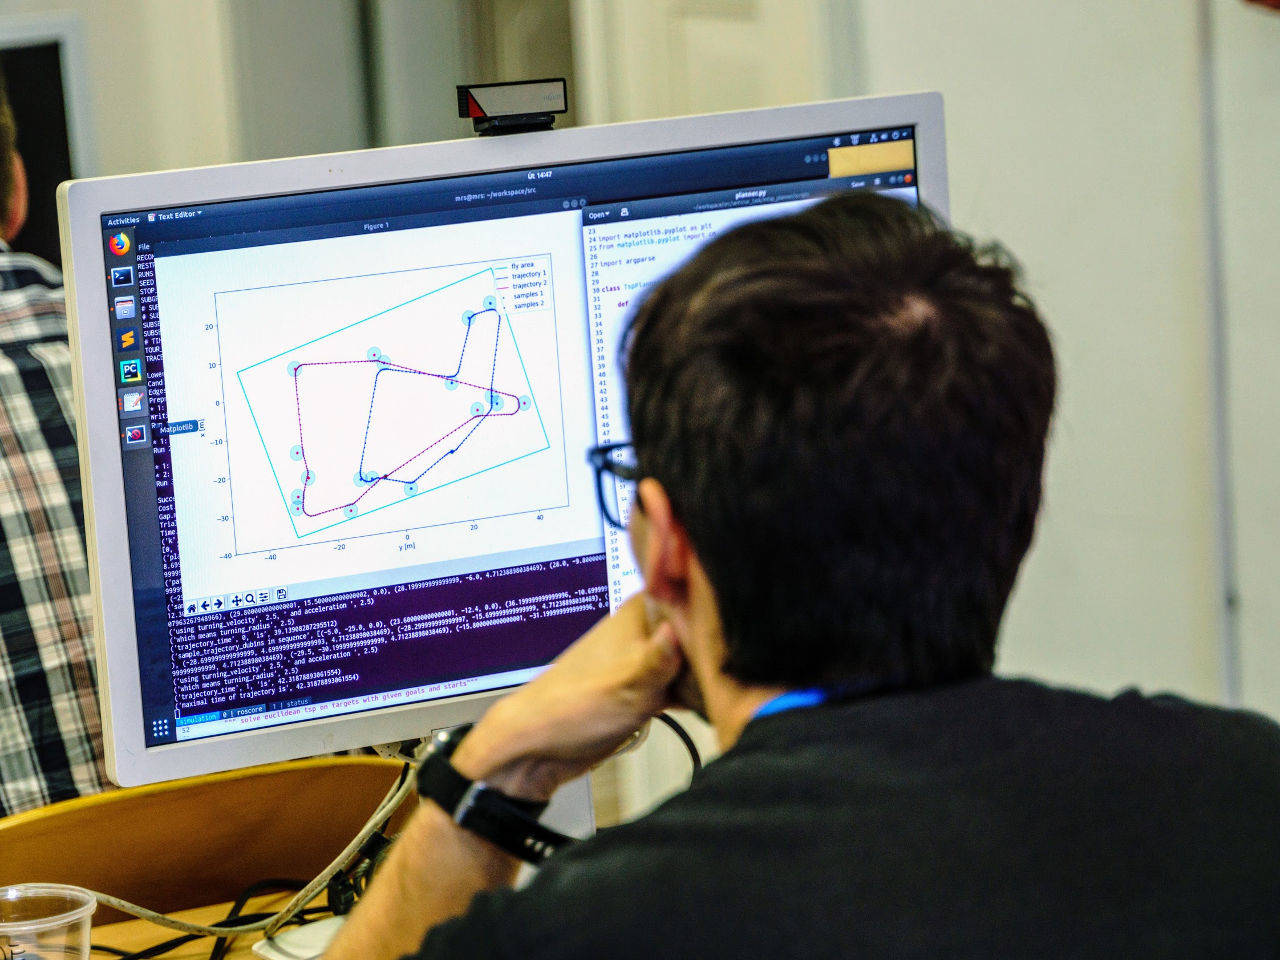
\includegraphics[width=0.235\textwidth]{./fig/photos/summer_schoo_pc.jpg}};
    \begin{scope}[x={(a.south east)},y={(a.north west)}]
      %%{ grid
      % % useful grid to help you find coordinates for plotting the overlay
      % \draw[black, xstep=.1, ystep=.1] (0,0) grid (1,1);
      % \foreach \i in {0,0.1,0.2,0.3,0.4,0.5,0.6,0.7,0.8,0.9,1} {
      %   \node[align=center] at (\i, -0.05) {\i};
      %   \node[align=center] at (\i, 1.05) {\i};
      %   \node[align=center] at (-0.05, \i) {\i};
      %   \node[align=center] at (1.05, \i) {\i};
      % }
      %%}
      % plot some stuff over the image
      \fill[white] (0.001, 0.001) rectangle (0.12,0.13);
      \fill[draw=black, draw opacity=0.5, fill opacity=0] (0,0) rectangle (1, 1);
      \node[imgletter,text=black] (label) at (a.south west) {(a)};
    \end{scope}
  \end{tikzpicture}}
  \hfill%
  \subfloat {\begin{tikzpicture}
    \node[anchor=south west,inner sep=0] (a) at (0,0) { 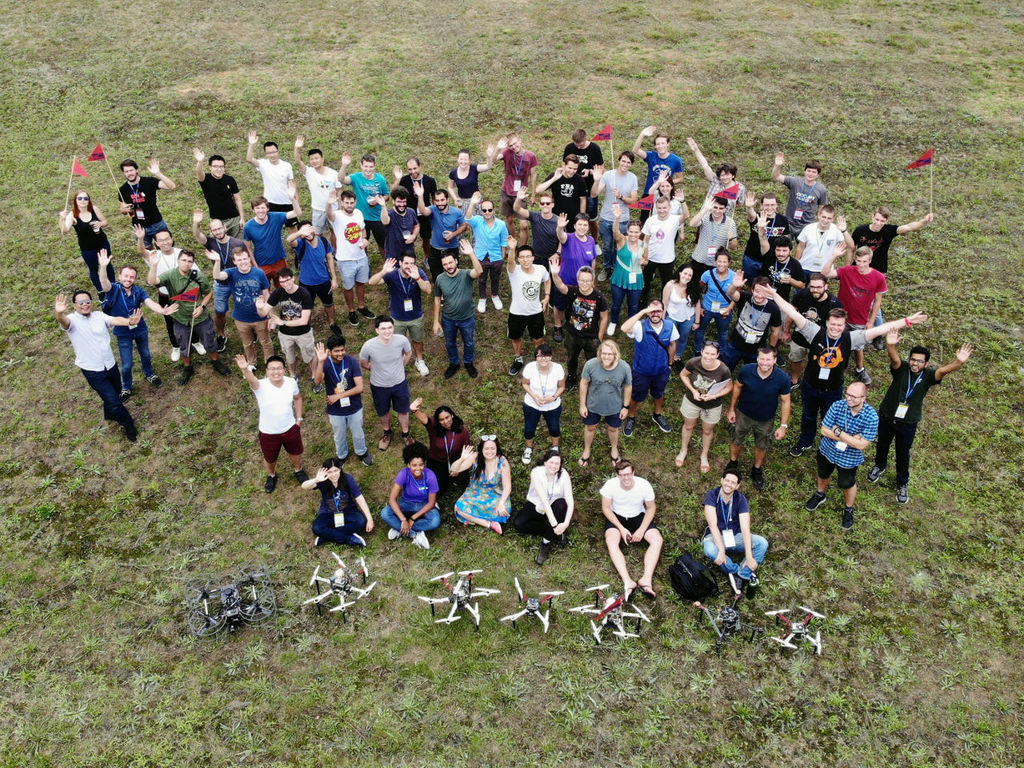
\includegraphics[width=0.235\textwidth]{./fig/photos/summer_school_outdoor.jpg}};
    \begin{scope}[x={(a.south east)},y={(a.north west)}]
      %%{ grid
      % % useful grid to help you find coordinates for plotting the overlay
      % \draw[black, xstep=.1, ystep=.1] (0,0) grid (1,1);
      % \foreach \i in {0,0.1,0.2,0.3,0.4,0.5,0.6,0.7,0.8,0.9,1} {
      %   \node[align=center] at (\i, -0.05) {\i};
      %   \node[align=center] at (\i, 1.05) {\i};
      %   \node[align=center] at (-0.05, \i) {\i};
      %   \node[align=center] at (1.05, \i) {\i};
      % }
      %%}
      % plot some stuff over the image
      \fill[white] (0.001, 0.001) rectangle (0.12,0.13);
      \fill[draw=black, draw opacity=0.5, fill opacity=0] (0,0) rectangle (1, 1);
      \node[imgletter,text=black] (label) at (a.south west) {(b)};
    \end{scope}
  \end{tikzpicture}}
  \caption{The 2019 IEEE RAS summer school on multirobot systems organized theoretical lectures, (a) exercises with the proposed system, and (b) a practical experimental session, in which students competed in an automatic planning challenge. Go to \protect\url{http://youtu.be/m_AxZs-_DXI} for a summary video from the event.}
  \label{fig:summer_school_2019}
\end{figure}

%%}

%%}

%% | ------------------------ Chapter 5 ----------------------- |

%%{ Ionizing Radiation Detection and Localization by UAVs

\chapternoclear{Ionizing Radiation Detection and Localization by UAVs}
\chaptermark{Ionizing Radiation Localization}

Ongoing research realized in the accepted TACR 2020-2022 project FW01010317:\\
``\textit{Lokalizace zdrojů ionizující radiace pomocí malých bezpilotních helikoptér s detektorem na principu Comptonovy kamery}''.

Relevant author's publications (will be discussed):
\fullciteinbox{baca2016miniaturized}{}
\fullciteinbox{baca2018timepix}{}

Author's publications to be included in the thesis:
\includepaper{baca2018timepix}
\includepaper{baca2019timepix}
\includepaper{stibinger2020localization}

Related author's publications: \cite{baca2016miniaturized, urban2017vzlusat}

%%{ Introduction

\section{INTRODUCTION}

Localization of ionizing radiation sources has recently become the domain of autonomous mobile robots.
Following the 2011 disaster at the \ac{FDNPP}, considerable efforts went into minimizing the exposure of human workers by sending \acp{UGV} into potentially hazardous areas.
Mapping a radiation distribution within an area is traditionally done with a dosimeter (measures intensity of radiation) while scanning the whole area.
On the other hand, the search for compact sources is better done with sensors capable of estimating the direction to the source.
The direction estimation is traditionally achieved by pixel radiation sensors (cameras) with sensor attachments, such as pinhole optics, coded apertures, and collimators \cite{baca2019timepix}.
In recent years, Compton cameras made an addition to the list of ways to estimate a set of directions to the source, however, without an external attachment to the sensor.
A \emph{traditional} Compton camera provides the direction to a source by measuring products of a Compton scattering reaction within two detectors (scatter and absorber).
Information on the products is used to calculate a set of possible directions to the source in the form of a cone surface in 3D.

%%{ Fig: drone and timepix

\begin{figure}
  \centering
  \subfloat {
    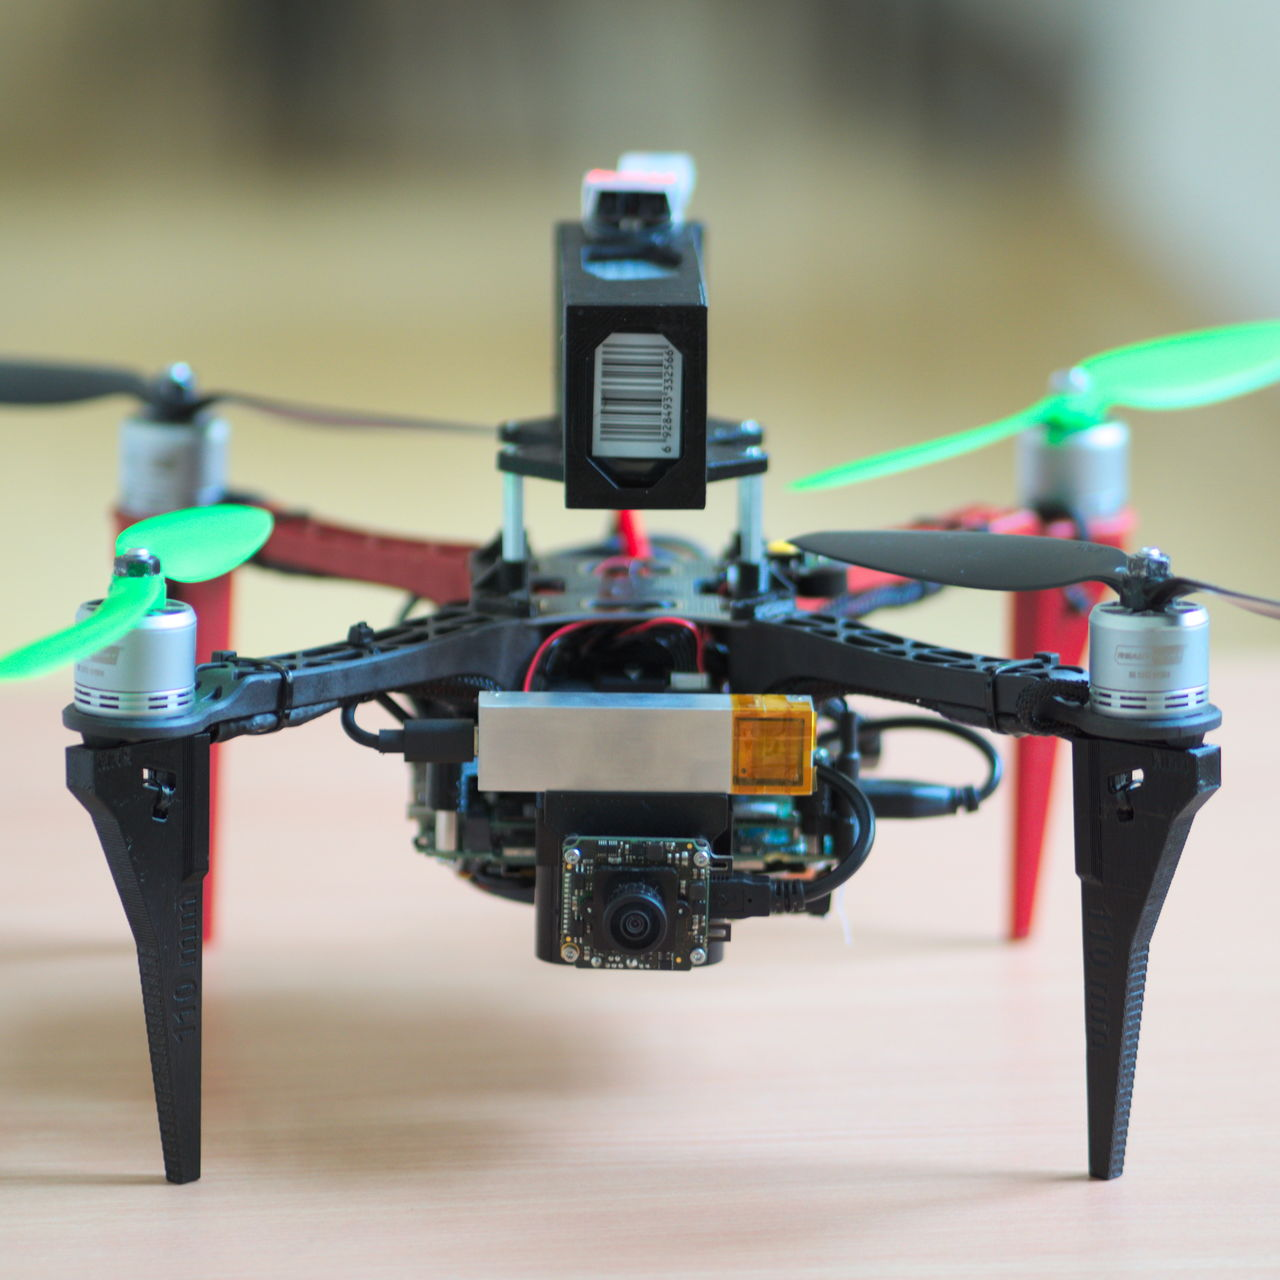
\includegraphics[width=0.390\textwidth]{./fig/photos/vio_drone.jpg}
  }%
  \subfloat {
    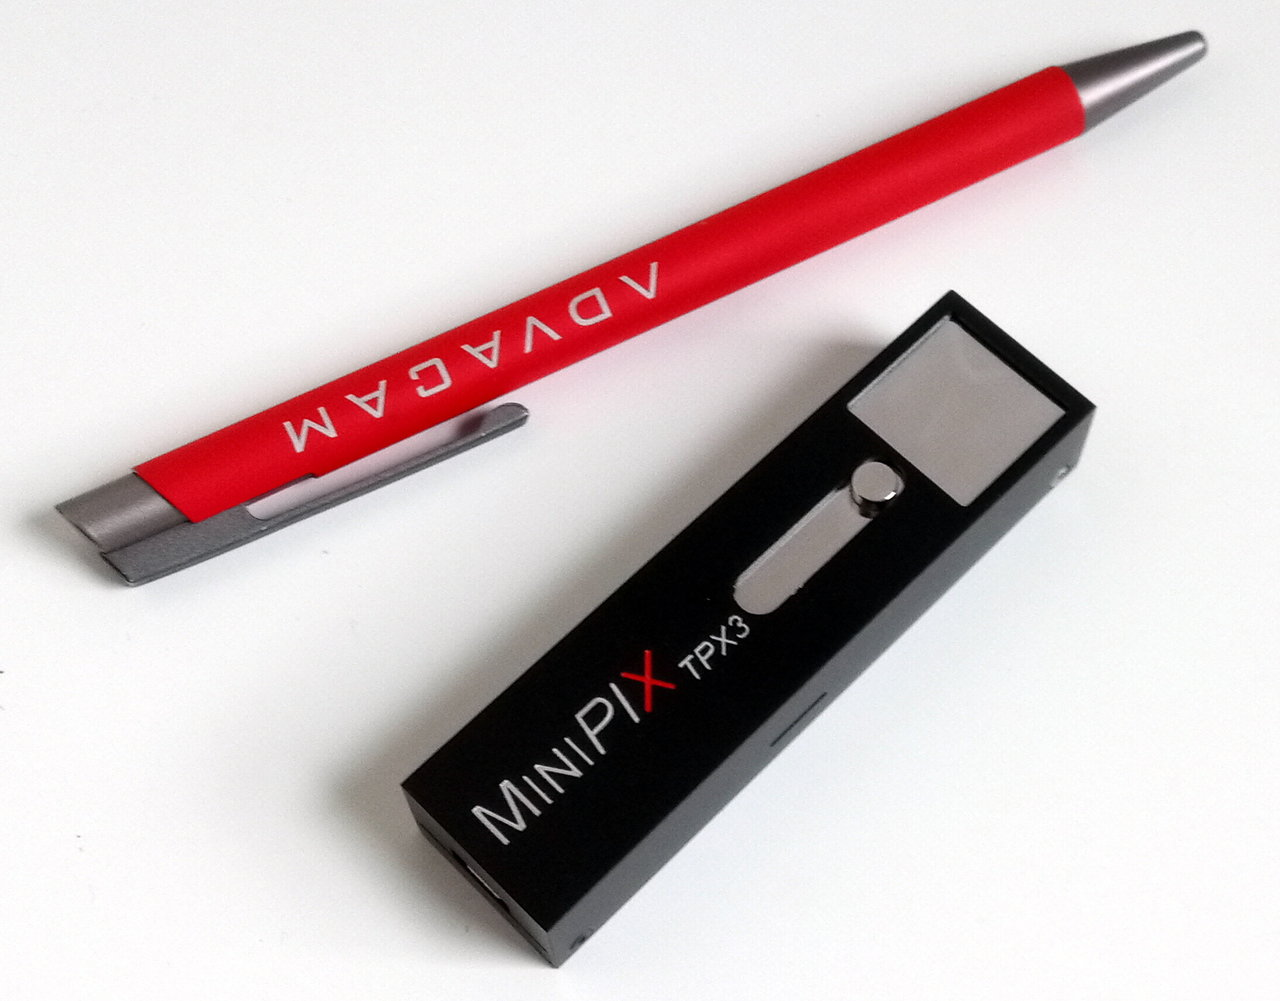
\includegraphics[width=0.50\textwidth]{./fig/photos/minipix_pen.jpg}
  }%
  \hfill%
  \caption{An \ac{MAV} with the mini MiniPIX Compton camera.}
  \label{fig:timepix}
\end{figure}

%%}

We aim to bring the Compton camera to the world of \acp{MAV} --- sub-\SI{250}{\gram} \acp{UAV}.
With current state-of-the-art technologies, \acp{MAV} can fly autonomously in cluttered environments, such as urban and indoor environments and forests.
An \ac{MAV} can pursue an informed exploration of the environment towards the estimated position of the source if such a real-time estimate is available.

%%{ Fig: Compton scattering

\begin{figure}[!b]
  \centering
  \resizebox{0.25\textwidth}{!}{%
    \begin{tikzpicture}[thick]
  \tikzset{snake it/.style={decorate, decoration=snake}}
    \draw[draw=red,snake it] (0.0, 0.0) -- (2.0, 0.0);
    \node at (0.0, 0.3) {$\lambda$};

    \draw[draw=green,snake it] (2.0, 0.0) -- (3.414, 1.414);
    \node at (3.614, 1.414) {$\lambda'$};

    \draw[draw=black,dashed] (2.0, 0.0) -- (3.0, 0.0);

    \draw[->, draw=black] (2.0, 0.0) -- (3.0, -0.5);
    \node at (3.2, -0.5) {$e^{\minus}$};

    \draw[black, dashed] (3,0) arc (0:40:1);
    \node at (2.7, 0.25) {$\Theta$};

    \fill[circle,shading=ball,outer color=gray!30] (2.0,0) circle (5pt);
\end{tikzpicture}

  }
  \caption{
    Compton scattering: an incoming gamma photon $\lambda$ changes its momentum as it scatters off a scattering center by a scattering angle $\Theta$.
    The decrease in momentum creates an electron.
  }
  \label{fig:compton_scattering}
\end{figure}

%%}

%%{ Sub: Related works

\subsection{Related work}

% In the field of radiation sensing, unmanned robotic vehicles offer several advantages over conventional handheld detectors or piloted aircraft.
% These advantages can be exploited in a wide variety of applications.

% Following the 2011 disaster at the \ac{FDNPP}, considerable amounts of radioactive material have been released into the plant area.

Several \acp{UGV} have been deployed directly inside the damaged reactor buildings of \ac{FDNPP} under remote control.
Various radiation detection methods have been tested inside the power plant, including a coded aperture scintillator \cite{ohno2011robotic}, a semiconductor digital dosimeter \cite{nagatani2013emergency}, a Compton event camera composed of two scintillators \cite{sato2019radiation}, and a time-of-flight gamma camera \cite{kinoshita2014development}.
Ground-based robots offer higher payload capacity and the ability to carry heavier sensory equipment than most aerial vehicles.
On the other hand, these robots tend to be relatively bulky, struggle to navigate the cluttered corridors and staircases inside the damaged buildings, and generally move slower than a multirotor aircraft.

\acp{UAV} have been utilized to map the spread of the radioactive material outside of the power plant.
These range from large aircraft weighing more than \SI{90}{\kilogram} equipped with heavy scintillation detectors \cite{sanada2015aerial, towler2012radiation, jiang2016prototype}
to compact multi-rotors suitable for flying along a pre-defined trajectory close to the ground \cite{macfarlane2014lightweight, christie2017radiation, martin20163d}.
Outside of Japan, several projects have employed \acp{UAV} for radiation intensity mapping around uranium ore mines \cite{salek2018mapping, keatley2018source, martin2015use}.

In \cite{han2013lowcost}, multiple fixed-wing \acp{UAV} equipped with miniature scintillators are used for contour analysis of an irradiated area.
Trajectory planning and data processing are performed offline, contrary to our approach, which estimates the position of the source in real-time during the flight.
In \cite{newaz2016uav}, the contour analysis is tackled using a single multirotor \ac{UAV}. The contour analysis uses a Gaussian mixture model to estimate multiple radiation sources' positions with overlapping intensity fields.
The projects mentioned above utilize unmanned vehicles to deliver a radiation sensor into a hazardous environment.
However, the approaches do not respond to measured data in real-time and thus do not exploit the mobility of \acp{UAV} to improve the measurement.

Active path-planning driven by the onboard measurements has been shown in \cite{towler2012radiation} for an outdoor environment and in \cite{mascarich2018radiation} for a GPS-denied indoor environment.
Both of these works rely on a scintillator sensor to estimate the radiation intensity in the \ac{UAV}'s current position.
As a result, the employed aerial platforms have to be large with a payload capacity exceeding \SI{2}{\kilogram}.
As in \cite{towler2012radiation}, the aerial platform is a \SI{90}{\kilogram} unmanned aerial helicopter, which significantly limits its deployment conditions due to personal safety and considerable minimum distance to obstacles in the environment.

The lack of lightweight radiation detectors with immediate readout capability severely limits the application potential of aerial dosimetry.
However, a new robotic methodology for motion planning and exploration needs to be developed to accommodate the proposed measurement system's specifics.
The proposed system is intended for outdoor and indoor environments, prompting a very compact and self-sufficient vehicle.
We build upon our previous experience with indoor \ac{UAV} deployment \cite{baca2020mrs}, where such radiation localization system could be used during exploration of mine shafts and caves \cite{roucek2019darpa, petrlik2020robust}, in interiors of large buildings \cite{kratky2020autonomous, saska2020formation}, in forests \cite{petracek2020bioinspired} and in nuclear power plants \cite{kratky2020autonomous2}.

%%}

%%{ Tab: nomenclature

\begin{table*}
  \scriptsize
  \centering
  \noindent\rule{\textwidth}{0.5pt}
  \begin{tabular}{lll}
    $\mathbf{x}$, $\bm{\alpha}$ & vector, pseudo-vector, or tuple\\
    $\mathbf{\hat{x}}$, $\bm{\hat{\omega}}$& unit vector or unit pseudo-vector\\
    $\mathbf{\hat{e}}_1, \mathbf{\hat{e}}_2, \mathbf{\hat{e}}_3$ & elements of the \emph{standard basis} \\
    $\mathbf{X}, \bm{\Omega}$ & matrix \\
    $x = \mathbf{a}^\intercal\mathbf{b}$ & inner product of $\mathbf{a}$, $\mathbf{b}$ $\in \mathbb{R}^n$\\
    $\mathbf{x} = \mathbf{a}\times\mathbf{b}$ & cross product of $\mathbf{a}$, $\mathbf{b}$ $\in \mathbb{R}^3$\\
  \end{tabular}%
  \begin{tabular}{lll}
    $\mathbf{x} = \mathbf{a}\circ\mathbf{b}$ & element-wise product of $\mathbf{a}$, $\mathbf{b}$ $\in \mathbb{R}^n$ \\
    $x_{[n]}$ & $x$ at the sample $n$ \\
    $\mathbf{A}, \mathbf{x}, \mathbf{\Omega}$ & LKF system matrix, state vector, covariance\\
    $\Delta t$ & time difference interval, [\si{\second}] \\
    $\mathbf{x}_\mathcal{B}, \mathbf{x}_\mathcal{W}, \mathbf{x}_\mathcal{C}$ & $\mathbf{x}$ in body-fixed, world, and camera frame \\
    $\angle\left(\mathbf{a}, \mathbf{b}\right)$ & signed angle between vectors (right-hand rule) \\
  \end{tabular}
  \noindent\rule{\textwidth}{0.5pt}
  \caption{Mathematical notation, nomenclature, and notable symbols.}
  \label{tab:nomenclature}
\end{table*}

%%}

%%{ Sub: Contributions

\subsection{Contributions}

We present a novel system for gamma source radiation localization using a single-sensor Compton camera \cite{turecek2020single}.
The system utilizes an onboard position estimator of a \ac{UAV} to create a real-time hypothesis of the radiation source position.
The proposed method is executed in real-time such that the results can be used to drive an autonomous search algorithm.
Unlike any existing solution, the system is deployable onboard \aclp{MAV} thanks to the small form factor of the Compton camera sensor.
The proposed approach is intended as an addition to an intensity-based estimation approach.
The used MiniPIX TPX3 CdTe sensor with \ac{CdTe} detector can also detect $\beta$ and heavy-ion radiation and, therefore, can be used without changes to estimate gradients and contours of radiation intensity.
Even more, particle tracks can be classified \cite{baca2019timepix} to deduce the nature of the radiation source.

%%}

%%}

%%{ Compton camera

\section{TIMEPIX3 COMPTON CAMERA}

%%{ Fig: Coordinate frames

\begin{figure}
  \centering
  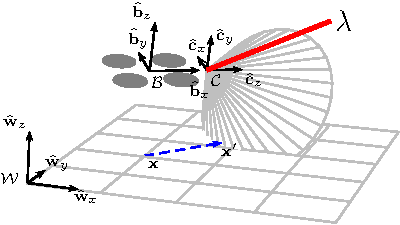
\includegraphics[width=0.35\textwidth]{./fig/sketch/coordinate_frames.pdf}
  \caption{
    Compton camera coordinate frame $\mathcal{C}$ is attached to the \ac{UAV} body frame $\mathcal{B}$.
    The world coordinate frame $\mathcal{W}$ is static. Transformations between the frames are provided by the \ac{UAV} control system \cite{baca2020mrs} through \ac{ROS}.
  }
  \label{fig:sketch_coordinate_frames}
\end{figure}

%%}

The process of recording and imaging ionizing gamma radiation is very different from the near-visible light spectrum photography \cite{baca2019timepix}.
Refractive optical lenses can not be made for such energies, and reflective optics (Kirkpatrick-Baez, Walter, Lobster-eye) are limited to energies no exceeding \SI{30}{\kilo\electronvolt} by the reflectivity of the used mirror materials such as gold and silicon.
Pinhole gamma cameras are a viable option.
However, their \ac{FOV} is narrow, and the aperture shield absorbs a valuable portion of the incoming particles.

Compton cameras use the Compton scattering effect (see \reffig{fig:compton_scattering}) to reconstruct a projection of a radioactive source \cite{turecek2018compton}.
Typically, a Compton camera consists of two sensors.
The first sensor, a \emph{scatterer}, witnesses the Compton scattering effect in its detector by capturing the bi-product of the reaction --- the electron $e^{-}$.
The electron is captured immediately upon its creation.
The second sensor is placed behind the first and is dedicated to capturing the scattered photon $\lambda'$ through the photo-electric effect.
When both detectors detect the scattering products, they simultaneously measure the energy and the 3D position of the particles.
According to Compton,~1923~\cite{compton1923quantum}, the relation of energies of the particles to the scattering angle $\Theta$ is modelled as
\begin{equation}
  E_{\lambda'} = \frac{E_{\lambda}}{1 + \left(E_{\lambda} / \left(m_e c^2\right)\right)\left(1 - \cos\Theta\right)},
  \label{eq:compton_formulae}
\end{equation}
where $E_{\lambda}, E_{\lambda'}$ are the energies of the incoming and scattered photon (\si{\joul}), $E_{e^{\minus}}$ is the energy of the electron (\si{\joul}), $m_e = 9.10938356\times10^{-31}\,$\si{\kilogram} is the electron rest mass, and $c = 299792458$\,\si{\meter\per\second} is the speed of light in vacuum.
Since Compton scattering is a radially symmetrical effect, the reconstruction of $\Theta$ yields a set of possible incoming directions that forms a cone surface.

Contrary to recent works \cite{sato2019radiation, jiang2016prototype, terzioglu2018compton}, we employ only a single sensor to measure the scattering products \cite{turecek2020single}.
Using cutting-edge innovations in the field of particle imaging, we employ the Timepix3 sensor \cite{poikela2014timepix3} as part of the MiniPIX TPX3 event camera with a thick \SI{2}{\milli\meter} \ac{CdTe} detector \footnote{\url{https://advacam.com/camera/minipix-tpx3}}.
The thick semiconductor detector is capable of causing the scattering effects, as well as capturing the products.
Thanks to the sensor's event camera operation mode, both bi-products are timed with sub-nanosecond accuracy, and the depth of the event within the detector is calculated.
In contrast with traditional frame-based cameras, event-driven cameras output a continuous stream of data generated by the active (hit) pixels.
A similar trend emerged in the visible-light camera field \cite{kueng2016low}.
Timepix3 promises a similar impact in the field of aerial radiation detection, as its essential properties are perfectly suited for dynamically flying \acp{MAV}.

The coincidence detection window is set to \SI{86}{\nano\second}, which is the maximum time difference of two coinciding particles being measured at the opposite side of the \SI{2}{\milli\meter} \ac{CdTe} at \SI{450}{\volt}.
The detection window is specific to this particular detector and should be adjusted for different thicknesses, materials, and bias voltages.

\subsection{Reconstructing the set of directions to the source}

%%{ Fig: 3D Compton scattering

\begin{figure}
  \centering
  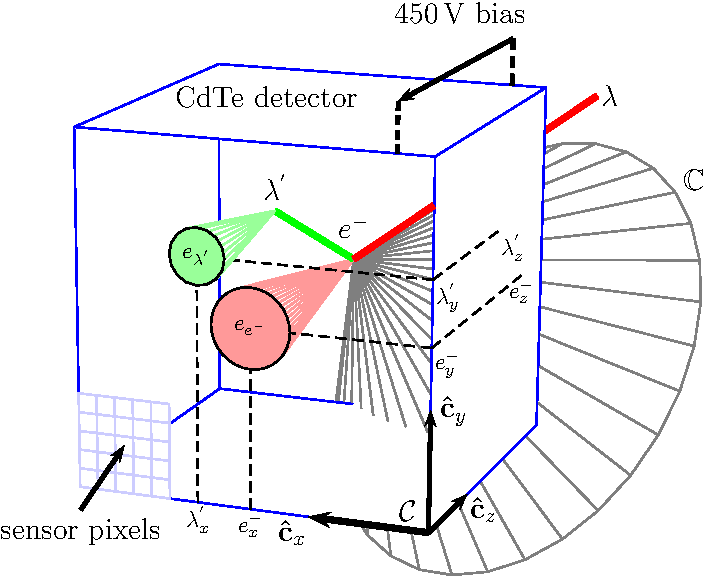
\includegraphics[width=0.30\textwidth]{./fig/sketch/compton_3d.pdf}
  \caption{
    An illustration of the Compton scattering effect within the \ac{CdTe} detector on top of the Timepix3 sensor.
    The ionized electron clouds are produced by absorption $\lambda'$ and $e^-$ and are gathered towards the sensor pixels by $\SI{450}{\volt}$ bias potential with a speed of $\approx$\,\SI{23}{\micro\meter\per\nano\second}.
  }
  \label{fig:3d_cone_reconstruction}
\end{figure}

%%}

Table~\ref{tab:nomenclature} summarizes the mathematical notation used throughout this work and \reffig{fig:sketch_coordinate_frames} provides an illustration of the used coordinate systems.
Ionizing radiation separates electrons (ionization) from the \ac{CdTe} detector material in the location of absorption.
The newly created electron cloud is accelerated by a \SI{450}{\volt} electric potential towards one facet of the \SI{2}{\milli\meter} \ac{CdTe} detector where the charge is measured by individual pixels of the Timepix3 sensor.
Figure \ref{fig:3d_cone_reconstruction} shows the charge-gathering process within the detector.
The $[\lambda'_x, \lambda'_y]^\intercal_\mathcal{C}$ and $[e^{\minus}_x, e^{\minus}_y]^\intercal_\mathcal{C}$ coordinates of the events are obtained by calculating the centroids of the respective pixel tracks (see \reffig{fig:timepix_image}).
The z-coordinates $\lambda'_z$ and $e^{\minus}_z$ are unknown.
However, it is possible to estimate the relative difference along the $\mathbf{\hat{c}}_z$ using the measured time-difference of the events.
Although the absorption of $\lambda'$ and $e^{\minus}$ happens virtually at the same time\footnote{The speed of a gamma photon through \ac{CdTe} material is near the speed of light in vacuum and therefore can be neglected.}, the charge-gathering causes a delay between the measured electron clouds.
The relative z-distance is obtained as
\begin{equation}
  \Delta z = 2325.6\,(e^{\minus}_t - \lambda'_t),
\end{equation}
where $e^{\minus}_t$ and $\lambda'_t$ are the times of arrival of the electron clouds from the electron and photon, respectively, and $c_s$~=~\SI{23.256}{\micro\meter\per\nano\second}~=~\SI{2325.6}{\meter\per\second} is the charge-gathering speed through the \ac{CdTe} detector with \SI{450}{\volt} bias\footnote{The charge gathering speed is obtained empirically by analyzing tracks of muons from a cosmic radiation.}.
The absence of a precise absolute z-axis coordinate of the cone origin within the camera frame is inconsequential.
It results only in a shift of the resulting cone surface, which can be neglected compared to the real-world distances involved.
Only the difference between the scattering products along $\mathbf{\hat{c}}_z$ is significant for estimating the cone parameters.
Therefore, coordinates of the electron and the secondary photon events in the camera frame $\mathcal{C}$ are considered as
\begin{align*}
  \mathbf{e}^{\minus}_{\mathcal{C}} &= [e^{\minus}_x, e^{\minus}_y, \Delta z]^\intercal,\numberthis\\
  \bm{\lambda}'_\mathcal{C} &= [\lambda'_x, \lambda'_x, 0]^\intercal.\numberthis
\end{align*}

In order to reconstruct the scattering angle $\Theta$, we convert the measured particle energies from (\si{\kilo\electronvolt}) to (\si{\joul}) as
\begin{align*}
  E_{e^{\minus}} &= e_{e^{\minus}}/6.242\times10^{18},\numberthis\\
  E_{\lambda} &= e_{\lambda}/6.242\times10^{18},\numberthis
\end{align*}
and calculate the scattering angle using (\ref{eq:compton_formulae}) as:
\begin{align*}
  \Theta = \cos^{-1} \underbrace{\left(1 + m_e c^2 \left(\frac{1}{E_{e^{-}} + E_\lambda} - \frac{1}{E_\lambda}\right)\right)}_{B},\\\text{for}\ \minus 1 < B < 1\numberthis
  \label{eq:theta_equation}
\end{align*}
Finally, the cone parameters are the cone origin $\mathbf{o}_{\mathcal{C}} = \mathbf{e}^{\minus}$, the direction $\mathbf{\hat{d}}_\mathcal{C} = \mathbf{e}^{\minus} - \bm{\lambda}'$, and the inner angle $\Theta$.

%%{ Fig: Timepix images

\begin{figure}
  \centering
  \begin{tikzpicture}
    \node[anchor=south west,inner sep=0] (a) at (0,0) {
        \begin{tabular}{cc}
            \fbox{
\includegraphics[width=0.20\textwidth]{./fig/rviz/timepix_10s.png}}
          &
            \fbox{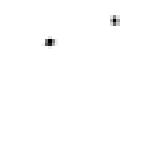
\includegraphics[width=0.20\textwidth]{./fig/rviz/timepix_10s_compton_zoom.png}}
        \end{tabular}
      };

    %%{ labels

    \begin{scope}[x={(a.south east)},y={(a.north west)}]

      \draw (0.37, 0.11) rectangle (0.43, 0.20);
      \draw[black] (0.43, 0.11) -- (0.525, 0.005);
      \draw[black] (0.43, 0.20) -- (0.525, 0.995);

      \draw (0.66,0.80) node [text=black] {\small photon track};
      \draw (0.83,0.95) node [text=black] {\small electron track};

      \draw (0.75,0.33) node [text=black] {
        \begin{tabular}{rl}
          \small $\lambda'_e$ = &\SI{394.22}{\kilo\electronvolt}\\
          \small $e^{\minus}_e$ = &\SI{315.70}{\kilo\electronvolt}\\
          \small $\Delta t$ = &\SI{20.31}{\nano\second}\\
          \small $\Delta z$ = &\SI{0.47}{\milli\meter}\\
          \hline
          \small $\Theta$ = &\SI{1.13}{\radian}\\
        \end{tabular}
      };

      %%{ grid

      % useful grid to help you find coordinates for plotting the overlay
      % \draw[black, xstep=.1, ystep=.1] (0,0) grid (1,1);
      % \foreach \i in {0,0.1,0.2,0.3,0.4,0.5,0.6,0.7,0.8,0.9,1} {
      %   \node[align=center] at (\i, -0.05) {\i};
      %   \node[align=center] at (\i, 1.05) {\i};
      %   \node[align=center] at (-0.05, \i) {\i};
      %   \node[align=center] at (1.05, \i) {\i};
      % }

      %%}

    \end{scope}

    %%}
  \end{tikzpicture}
  \caption{
    An example of a pair of Compton scattering products captured by the Timepix3 sensor.
    The events' times are used together with the particles' energies to reconstruct the scattering angle, $\Theta$.
  }
  \label{fig:timepix_image}
\end{figure}

%%}

%%}

%%{ Radiation source state estimation

\section{RADIATION SOURCE STATE ESTIMATION}

Estimating the direction to the source is typically done under assumptions that do not apply in scenarios involving mobile robots.
The camera position is often fixed during the whole measurement, and all the data are processed at once after the measurement \cite{turecek2018compton, terzioglu2018compton}.
In other cases, the camera needs to be stationary to complete a single measurement set (tens of seconds) before it can be moved further \cite{sato2019radiation, jiang2016prototype}.
However, the estimation should be conducted continuously without stopping to utilize the advantages of multirotor helicopters fully.
Moreover, in all the previous works involving a mobile robot, the used camera was a heavy device, which required the use of a large \ac{UGV} or \ac{UAV}.
We aim to bring the Compton camera sensor to the domain of \acp{MAV}.
With appropriate onboard localization and mapping systems, such \ac{MAV} can automatically perform the search for an ionizing radiation source.
However, this requires the \ac{MAV} to automatically estimate the source's position onboard in real-time to incorporate newly acquired data on the fly.
Here we present our initial method developed for a single radiation source localization.

The proposed method relies on the \ac{LKF} to estimate a hypothesis and a covariance of the source's position.
However, the \ac{LKF} is not natively able to accept the measured cone surfaces as a vector of measurement.
To tackle this issue, we assume that the optimal correction would move the hypothesis orthogonally in the cone surface direction.
Such corrections behave idempotently under ideal conditions.
Applying such a correction requires a novel approach of using \ac{LKF} by defining an orthogonal projection to the cone surface.

%%{ Sub: Orthogonal projection to a cone surface

\subsection{Orthogonal projection to a cone surface}

Projecting the \ac{LKF} hypothesis $\mathbf{x}_\mathcal{W}$ orthogonally to the cone surface to obtain ${\mathbf{x}'}_\mathcal{W}$ is illustrated in \reffig{fig:orthogonal_projection}.
Vector from the origin of the cone $\mathbf{o}_\mathcal{W}$ to the given point $\mathbf{x}_\mathcal{W}$ is denoted as $\mathbf{\hat{u}} = (\mathbf{x} - \mathbf{o})/\|\mathbf{x} - \mathbf{o}\|$.
Firstly, we find the angle between the cone direction $\mathbf{\hat{d}}$ and $\mathbf{\hat{u}}$ as $\alpha = \angle(\mathbf{\hat{u}}, \mathbf{\hat{d}})$.
Then, the angle between the cone surface and the desired orthogonal projection of $\mathbf{x}$ to the cone surface is $\beta = \alpha - \Theta$.
To find the projection, we first find $\mathbf{x}_r$ by rotating $\mathbf{x}$ around the vector $\mathbf{\hat{d}} \times \mathbf{\hat{u}}$ by the angle $\beta$.
The vector towards the projection is then constructed as $\mathbf{\hat{v}} = (\mathbf{x}_r - \mathbf{o})/\|\mathbf{x}_r - \mathbf{o}\|$.
Finally, the orthogonal projection of $\mathbf{x}$ on the cone surface is:
\begin{equation}
  \mathbf{x}' = \begin{cases}
    \mathbf{o} + \mathbf{\hat{v}}\cos\beta, & \text{if}\ \alpha < \pi/2,\\
    \mathbf{o}, & \text{if}\ \pi/2 \leq \alpha.
  \end{cases}
\end{equation}

%%{ Fig: Orthogonal projection

\begin{figure}
  \centering
  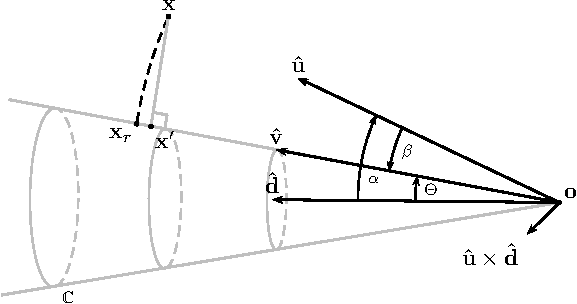
\includegraphics[width=0.35\textwidth]{./fig/sketch/orthogonal_projection.pdf}
  \caption{Orthogonal projection of $\mathbf{x}$ to the cone surface.}
  \label{fig:orthogonal_projection}
\end{figure}

%%}


%%}

%%{ Sub: LKF

\subsection{Linear Kalman Filter}

\acp{LKF} filter uses a model with the hypothesis $\mathbf{x}_{[t]}$ and hypothesis covariance $\mathbf{\Omega}_{[t]}$:
\begin{equation}
  \mathbf{x}_{[t]} = \m{A}\mathbf{x}_{[t-1]},~\mathbf{A} = \left[\begin{smallmatrix}
    1 & 0 & 0\\
    0 & 1 & 0\\
    0 & 0 & 1
  \end{smallmatrix}\right],
  \label{eq:lti_model}
\end{equation}
where $\mathbf{A}$ is designed for a stationary 3D target.
Measurement noise covariance with the correction being applied in the direction of the $\mathbf{\hat{e}}_3$ axis is defined as
\begin{equation}
  \mathbf{R_e} = \left[\begin{smallmatrix}
    r & 0 & 0 \\
    0 & 10^9 & 0 \\
    0 & 0 & 10^9
  \end{smallmatrix}\right],
\end{equation}
where $r$ is used to weight the correction in the direction to the cone surface.
The rest of the matrix is designed to mitigate corrections for other directions.
This canonical covariance $\mathbf{R}_e$ is then rotated every time to align with the vector $\mathbf{x}' - \mathbf{x}$ as $\mathbf{R} = \mathbf{P}\mathbf{R_e}\mathbf{P}^{\intercal}$
where $\mathbf{P}$ is a rotation matrix corresponding to rotation around the axis $\mathbf{\hat{e}}_3 \times \left(\mathbf{x}' - \mathbf{x}\right)$ by the angle $\angle \left(\mathbf{x}' - \mathbf{x}, \mathbf{\hat{e}}_1\right)$.
An obtained measurement is then the projection $\mathbf{x}'$ and the covariance $\mathbf{R}$.

Two variants of the filter were tested:
the fully-3D approach presented above, and a simplified 2D approach in which we assume that the radiation source is located on the ground.
In the latter case, we project the hypothesis onto the ground plane after each correction.

Initialization of the \ac{LKF} hypothesis can not be done using the first arriving measurement as typical.
To tackle this issue, we first gather $N$ cone surfaces with different points of origin.
The gathering can be done using one of many exploration schemes, e.g., a traditional gradient-based exploration using particle intensity measurements as heuristics or flying a pre-determined sweeping path.
With the first $N$ cones measured, we initialize the filter by optimizing for a point $\mathbf{p}$, which has the minimum square distance to the cones' surfaces.
Firstly, we must define the distance to a cone surface.

%%}

%%{ Fig: experiment

\begin{figure*}[!ht]
  \centering
  \subfloat {
    \begin{tikzpicture}
      \node[anchor=south west,inner sep=0] (a) at (0,0) { 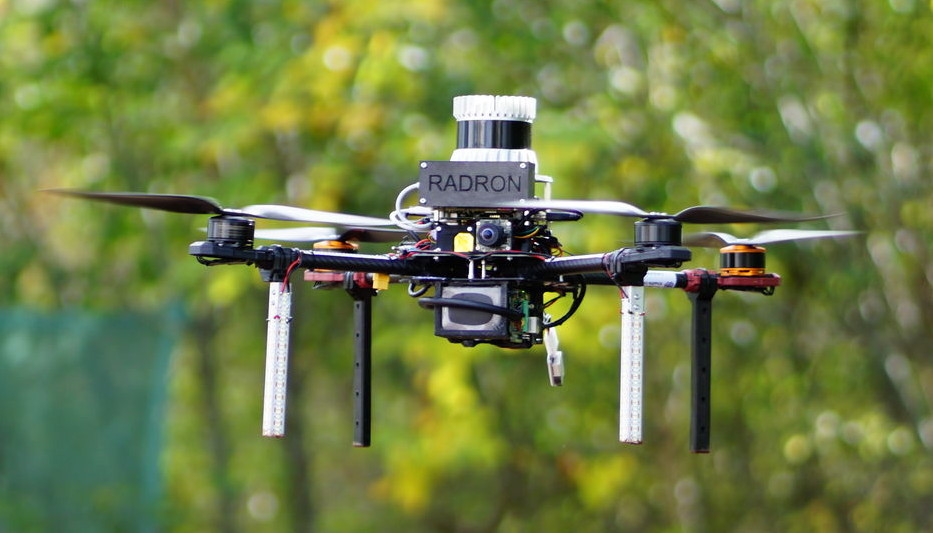
\includegraphics[width=0.31\textwidth]{./fig/photos/radron_uav.jpg}};
      \begin{scope}[x={(a.south east)},y={(a.north west)}]
        \node[imgletter] (letter) at (0.0, 0.0) {(a)};
        \draw (0.0, 0.0) rectangle (1.0, 1.0);
      \end{scope}
    \end{tikzpicture}
  }
  \subfloat {
    \begin{tikzpicture}
      \node[anchor=south west,inner sep=0] (a) at (0,0) { 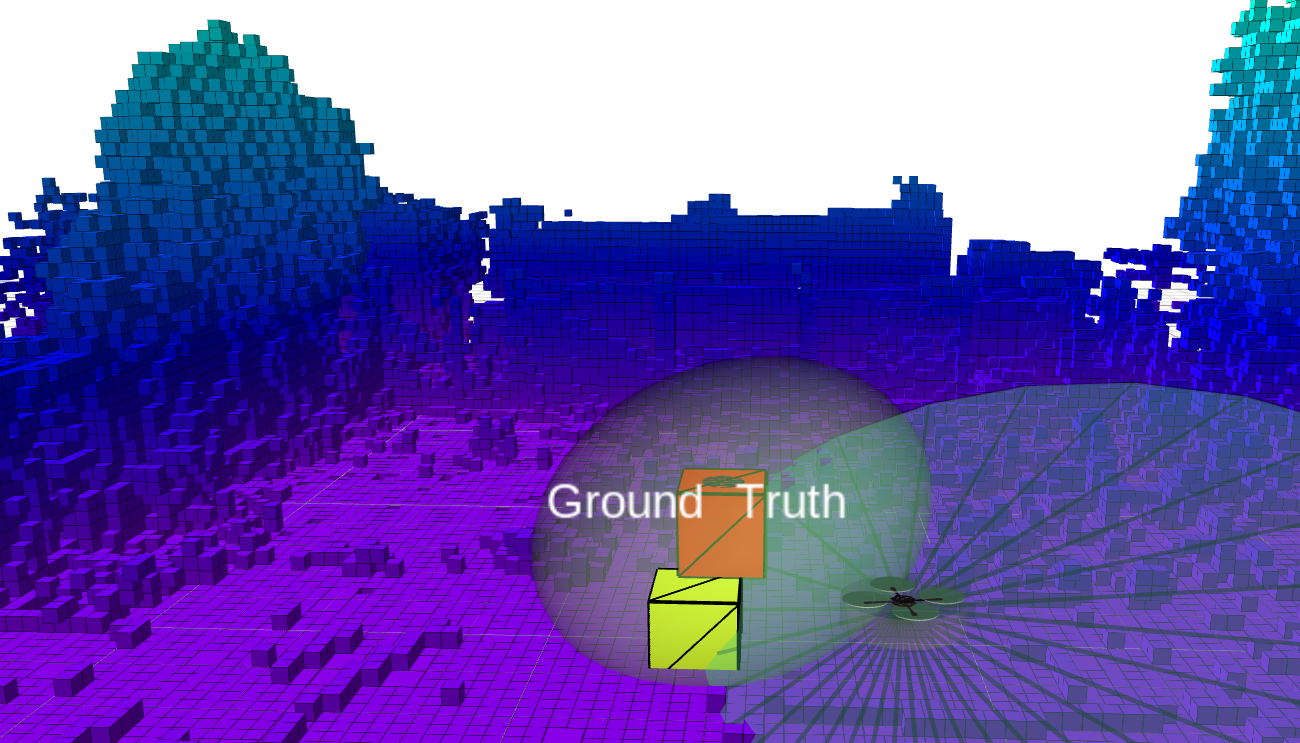
\includegraphics[width=0.31\textwidth]{./fig/rviz/rviz_3d.png}};
      \begin{scope}[x={(a.south east)},y={(a.north west)}]
        \node[imgletter] (letter) at (0.0, 0.0) {(b)};
        \draw (0.0, 0.0) rectangle (1.0, 1.0);
      \end{scope}
    \end{tikzpicture}
  }
  \subfloat {
    \begin{tikzpicture}
      \node[anchor=south west,inner sep=0] (a) at (0,0) { 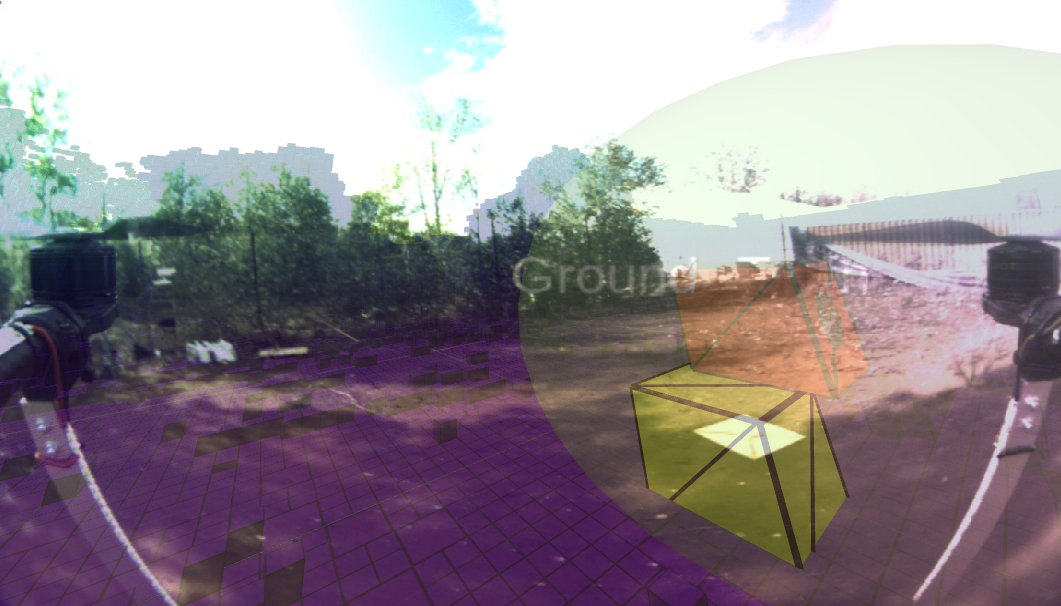
\includegraphics[width=0.31\textwidth]{./fig/rviz/bluefox_3d.png}};
      \begin{scope}[x={(a.south east)},y={(a.north west)}]
        \node[imgletter] (letter) at (0.0, 0.0) {(c)};
        \draw (0.0, 0.0) rectangle (1.0, 1.0);
      \end{scope}
    \end{tikzpicture}
  }
  \caption{
    The multi-rotor \ac{UAV} (a) was equipped with the MiniPIX TPX3 CdTe Compton camera, a 3D \ac{LiDAR}, and an RGB camera.
    \ac{SLAM} localizes the \ac{UAV} in 3D, which allows it to build a map of the surrounding environment (b).
    The RGB camera (c) serves for visual re-projection of the source's position.
    The estimated position of the source is shown in comparison with the ground truth position.
    Videos from the experiment are available at \url{http://mrs.felk.cvut.cz/radron-icra}.
  }
  \label{fig:experiment}
\end{figure*}

%%}

%%{ Sub: Distance to a cone surface

\subsection{Distance to a cone surface}

Given a point $\mathbf{p}$ such that $\text{if}\ \mathbf{\hat{d}}^{\intercal}_{i}\mathbf{p} < \mathbf{\hat{d}}_i^{\intercal}\mathbf{o}_i$ ($\mathbf{p}$ is situated \emph{behind} the cone origin), the distance to the cone surface is trivial:
\begin{equation}
  d(\mathbf{p}, \mathbf{o}, \mathbf{\hat{d}}, \Theta) = \|\mathbf{o} - \mathbf{p}\|.
\end{equation}
Otherwise, the distance is expressed as
\begin{equation}
  d(\mathbf{p}, \mathbf{o}, \mathbf{\hat{d}}, \Theta) = \|\mathbf{p} - \mathbf{o}\| \sin \left( \cos^{-1}\frac{\left(\mathbf{p} - \mathbf{o}\right) \circ \mathbf{\hat{d}}}{\|\mathbf{p} - \mathbf{o}\|} - \Theta\right).
\end{equation}

%%}

%%{ Sub: Finding the closest point to multiple cone surfaces

\subsection{Finding the closest point to multiple cone surfaces}

The state estimator's initialization is done by finding the closest point to the first \emph{N} cone surfaces.
The point $\mathbf{p}_\mathcal{W}$ is found by minimizing the squared distance to each cone surface while satisfying geometric constraints:
\begin{align*}
  & \min_{\mathbf{p} \in \mathbb{R}^3} \label{eq:mpc_cost}\numberthis
  & \sum_{i=1}^{N}d(\mathbf{p}, \mathbf{o}_i, \mathbf{\hat{d}}_i, \Theta_i)^2
\end{align*}\begin{align*}
  \text{s.t.}~ \mathbf{\hat{d}}^{\intercal}_{i}\mathbf{p} &\geq \mathbf{\hat{d}}_i^{\intercal}\mathbf{o}_i, &\forall i &\in \{1, \hdots, n\}\numberthis\label{eq:constraint_cone_halfspace},\\
  \mathbf{p}^\intercal\mathbf{\hat{e}}_3 &= 0, &\forall i &\in \{1, \hdots, n\}\numberthis\label{eq:constraint_ground_plane}.
\end{align*}
The constraint (\ref{eq:constraint_ground_plane}) is used optionally in the case of the 2D estimator to enforce the search for a source near the ground plane.

This optimization problem is a nonlinear least-squares problem, which makes finding a near-optimum solution impractical and time-consuming.
However, we do not need to solve this problem quickly or in fast succession, and the solution is used only for initialization.
Therefore, we utilize the Sequential Least-Squares Programming optimization method.
The Jacobian of the criterion is calculated analytically.
The problem takes approx. \SI{1}{\second} to solve for $N = 5$ on an average onboard computer.

%%}

%%}

%%{ Experiments

\section{EXPERIMENTS}

%%{ Fig: results

\begin{figure*}[!ht]
  \centering
  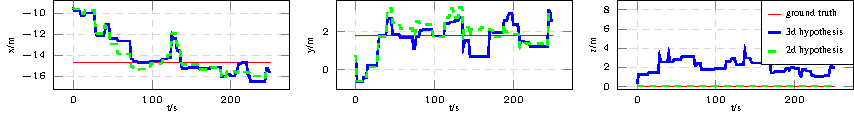
\includegraphics[width=1.0\textwidth]{./fig/plots/hypotheses.pdf}
  \caption{Plots of convergence of the 3D hypothesis and the 3D hypothesis in comparison to the ground truth.}
  % \vspace{-1em}
  \label{fig:results}
\end{figure*}

%%}

The approach was verified extensively in realistic simulations using the Gazebo/ROS simulator.
The Compton camera is modeled by combining real-time Monte-Carlo ray tracing and randomization of pre-computed Compton scattering products.
The Compton scattering products were pre-computed for a set of incident angles in the Geant4 particle physics simulator.
The obtained samples are then drawn randomly in real-time, given the relative incident angle between the source and the detector.
The data are as well augmented to create the radially-symmetrical ambiguity of the scattering.
Simulations suggest that the proposed methods are feasible.
However, the \ac{MAV} should conduct motion orthogonally to the direction of the source.
Otherwise, both the \ac{LKF} initialization and the \ac{LKF} correction methods result in singular solutions that fail to provide a full 3D position of the source.
However, such motion might be the only available option in urban areas if the source is placed behind a wall.

\subsection{Unmanned aerial vehicle}

The \ac{UAV} used for this demonstration is a general-purpose quadrotor helicopter built upon the Tarot 650 frame and equipped with Intel NUC-i7 onboard computer.
Figure \ref{fig:experiment}a depicts the \ac{UAV} in mid-air.
The Ouster OS1-16 3D \ac{LiDAR} was used for ground truth localization and mapping together with the A-LOAM \ac{SLAM} \cite{zhang2014loam}.
Furthermore, the \ac{UAV} was also equipped with a wide-angle RGB camera to aid with data visualization.
These sensors are not required for the proposed approach.
The only requirement is access to real-time 3D position and orientation state estimate of the \ac{UAV}.
Such a state estimate is a requirement for any autonomous mission.
It can be accommodated by, e.g., a \ac{GNSS} receiver coupled with an \ac{IMU} and magnetometer, or by a visual-inertial navigation system such as \cite{qin2018vins}.
Therefore, the Compton camera system can be employed on much smaller \ac{UAV} thanks to its small weight and size.
The design and size of the \ac{UAV} body is more limited by the localization sensor suite rather the by the \SI{40}{\gram} radiation sensor.
The \ac{UAV} utilized the open-source \emph{MRS UAV system}\footnote{\url{http://github.com/ctu-mrs/mrs_uav_system}}\cite{baca2020mrs} in \ac{ROS} for automatic control and state estimation.

\subsection{Compton camera sensor}

The Compton camera is built upon the Timepix3 sensor~\cite{poikela2014timepix3} with \SI{2}{\milli\meter} \ac{CdTe} detector.
\ac{CdTe} detectors are sensitive to high-energy gamma rays.
The exceptional sensitivity to high-energy $\gamma$ outweighs the small size (therefore small effective detector volume) of the detector since only high-energy $\gamma$ can travel hundreds of meters through the air without being absorbed.
This allows sensing the sources from a further distance than using traditional detectors.
The Timepix3 detector with thick \ac{CdTe} sensor can detect photons ranging from 5 to \SI{1000}{\kilo\electronvolt} with relatively high quantum efficiency especially for Compton scattering events.
The miniaturized Timepix3 based detector MiniPIX TPX3 \ac{CdTe} with incorporated data acquisition, calibration and event reconstruction software layers was developed by Advacam (see \reffig{fig:timepix}).
The device does not require any cooling and can operate at room temperature.
The Compton camera payload weighs \SI{40}{\gram} and has dimensions of $80 \times 20 \times 15$\,\si{\milli\meter}.
The processing software is implemented in \ac{ROS} and is available as open-source.

\subsection{Experimental environment}

These preliminary tests were conducted in $40 \times 20$\,\si{\meter} area with a single \isotope[137]{Cs} source with activity of \SI{187}{\mega\becquerel} ($187 \times 10^{6}$ decay events per second).
This was a relatively weak source, sending only $\approx\,$ \SI{30}{\per\second\per\centi\meter\squared} photons at \SI{10}{\meter} distance.
The presented experiment was conducted under autonomous localization, mapping, and control.
The control references were given by a human operator, and the \ac{UAV} followed the reference with \SI{1}{\meter\per\second} speed.
The \ac{UAV} first conducted a sweeping flight pattern while gathering the first 5 cone surfaces for initialization.
After the \ac{LKF} was initialized, it started encircling the current hypothesis.
Such a strategy shows success in simulations.
After successfully localizing the source, the estimator can adapt to the potentially changing position of the source.
Figure \ref{fig:experiment} depicts the 3D map of the environment with the hypothesis showed as a red cube surrounded by a covariance ellipsoid.
A yellow cube marks the ground truth position of the source.

\subsection{Results}

Figure \ref{fig:results} shows plots of the estimated 3D and 2D position of the gamma source in comparison to the ground truth.
The hypothesis was correctly estimated near the ground truth after gathering just 15 Compton events.
The experimental data show the estimator system working as expected.
Future work should emphasize rejecting outliers.
Outliers can occur due to the omnipresent radiation background.
However, despite the occasional outliers, the estimator performed well despite the tested radiation source's low activity.

%%}

%%{ Lessons learned and future work

  \section{LESSONS LEARNED AND FUTURE WORK}

  The presented results are a pilot work for a project for autonomous localization and tracking of compact ionizing radiation sources by \aclp{MAV}.
  Several significant challenges have been identified that are yet to be tackled before the solution becomes fully autonomous and reliable.
  The single-sensor Compton camera should be compared to a multi-sensor stack.
  Although the proposed single-sensor variant offers a significantly simpler hardware solution, the angular resolution is worse than with a sensor stack.
  Moreover, reconstruction of cone surfaces using (\ref{eq:theta_equation}) should benefit from outlier rejection using the values of $E_\lambda, E_{\lambda'}, E_{e^{-}}$.
  Priors of $E_\lambda$ can be estimated in real-time by analyzing the spectrum, a type of incoming particles.
  Also, the state estimation hypothesis should be generalized to a mixture of distributions.
  In combination with the observed complex 3D map of the environment, Monte-Carlo methods such as the particle filter should be explored.
  If available, prior knowledge of the environment structure, e.g., wall material and thickness, should also be utilized by the estimator.

  We pursue the use of \acp{MAV} equipped with monocular visual \ac{SLAM} (see \reffig{fig:timepix}).
  Autonomous planning methods should simultaneously explore an unknown environment while maximizing the yield of information gathered by the Compton camera.
  This task shares goals with the \ac{DARPA} SubT challenge\footnote{\url{https://www.subtchallenge.com}} in which the authors participate.
  Simulations show that the multi-\ac{MAV} system benefits significantly from sharing the measured data between the \acs{MAV} \cite{stibinger2020localization}.
  We aim to utilize swarms of \acp{MAV} to increase the \emph{baseline} of the distributed sensor, which increases the convergence speed of the estimator.

%%}

%%}

%% | ------------------------ Chapter 6 ----------------------- |

%%{ Conclusion

\chapternoclear{Conclusion}

\todo{}

%%}

%% | ----------------------- References ----------------------- |

%%{ References

\appendix
\renewcommand\chaptername{Appendix}

\chapternoclear{References}

Below are listed all publications of the author.
Each citation is displayed with percentage contribution of the author and number of citations based on Web of Science~(WoS), Scopus and Google Scholar~(GS).
\todo{updated citations}
% Journal articles also contains information about the Impact Factor~(IF) by Web of Science and the CiteScore~(CS) by Scopus.
% The publications~\cite{loianno2018localization, petrlik2020robust, stibinger2020localization, saikin2020wildfire} are only reported with CS due to the novelty of the journal that is expected to receive impact factor in June 2020.

\section{Thesis core publications}

\subsection*{Core articles in peer-reviewed journals}
\printbibliography[keyword={mine},keyword={phd_related},keyword={journal},keyword={core},notkeyword={submitted},heading=none,title={}]

\subsection*{Core conference proceedings}
\printbibliography[keyword={mine},keyword={phd_related},keyword={conference},keyword={core},notkeyword={submitted},heading=none,title={}]

\subsection*{Core articles --- submitted}
\printbibliography[keyword={mine},keyword={phd_related},keyword={submitted},keyword={core},heading=none,title={}]

\section{Thesis-related author's publications}

\subsection*{Thesis-related articles in peer-reviewed journals}
\printbibliography[keyword={mine},keyword={phd_related},keyword={journal},notkeyword={core},notkeyword={submitted},heading=none,title={}]

% \subsection*{Thesis-related articles in peer-reviewed journals only with CiteScore~(CS)}
% \printbibliography[keyword={mine},keyword={phd_related},keyword={journal},keyword={cs},heading=none,title={}]

\subsection*{Thesis-related conference proceedings}
\printbibliography[keyword={mine},keyword={phd_related},keyword={conference},notkeyword={core},notkeyword={submitted},heading=none,title={}]

\subsection*{Thesis-related publications --- submitted}
\printbibliography[keyword={mine},keyword={phd_related},keyword={submitted},notkeyword={core},heading=none,title={}]

\section{Partially-related author's publications}

\subsection*{Articles in peer-reviewed journals}
\printbibliography[keyword={mine},keyword={phd_unrelated},keyword={journal},notkeyword={core},notkeyword={submitted},heading=none,title={}]

\subsection*{Conference proceedings}
\printbibliography[keyword={mine},keyword={phd_unrelated},keyword={conference},notkeyword={core},notkeyword={submitted},heading=none,title={}]

\section{Cited references}
\printbibliography[notkeyword=mine,heading=none,title={}]

%%}

%% | ------------------------ Apendices ----------------------- |

%%{ Apendices

\appendix
\renewcommand\chaptername{Citations of author's publications}

\chapternoclear{Citations of author's publications}

Below are listed all citations of author's publications without self-citations.

\DeclareCiteCommand{\fullcite}
{\usebibmacro{prenote}}
{\clearfield{addendum}%
  \usedriver
  {\defcounter{minnames}{6}%
  \defcounter{maxnames}{6}}
{\thefield{entrytype}}}
{\multicitedelim}
{\usebibmacro{postnote}}

\noindent
\fullcite{saska2017system}
\begin{refsection}[citations/no_autocit/saska2017system.bib]
  \nocite{*}
  \printbibliography[heading=none,title={},env=favoritebib]
\end{refsection}

% \noindent
% \fullcite{faigl2017onsolution}
% \begin{refsection}[citations/no_autocit/faigl2017onsolution.bib]
%   \nocite{*}
%   \printbibliography[heading=none,title={},env=favoritebib]
% \end{refsection}

% \noindent
% \fullcite{saska2016formations}
% \begin{refsection}[citations/no_autocit/saska2016formations.bib]
%   \nocite{*}
%   \printbibliography[heading=none,title={},env=favoritebib]
% \end{refsection}

\noindent
\fullcite{baca2016miniaturized}
\begin{refsection}[citations/no_autocit/baca2016miniaturized.bib]
  \nocite{*}
  \printbibliography[heading=none,title={},env=favoritebib]
\end{refsection}

\noindent
\fullcite{loianno2018localization}
\begin{refsection}[citations/no_autocit/loianno2018localization.bib]
  \nocite{*}
  \printbibliography[heading=none,title={},env=favoritebib]
\end{refsection}

\noindent
\fullcite{spurny2019cooperative}
\begin{refsection}[citations/no_autocit/spurny2019cooperative.bib]
  \nocite{*}
  \printbibliography[heading=none,title={},env=favoritebib]
\end{refsection}

\noindent
\fullcite{daniel2016terrestrial}
\begin{refsection}[citations/no_autocit/daniel2016terrestrial.bib]
  \nocite{*}
  \printbibliography[heading=none,title={},env=favoritebib]
\end{refsection}

\noindent
\fullcite{baca2017autonomous}
\begin{refsection}[citations/no_autocit/baca2017autonomous.bib]
  \nocite{*}
  \printbibliography[heading=none,title={},env=favoritebib]
\end{refsection}

\noindent
\fullcite{baca2018model}
\begin{refsection}[citations/no_autocit/baca2018model.bib]
  \nocite{*}
  \printbibliography[heading=none,title={},env=favoritebib]
\end{refsection}

\noindent
\fullcite{daniel2017xray}
\begin{refsection}[citations/no_autocit/daniel2017xray.bib]
  \nocite{*}
  \printbibliography[heading=none,title={},env=favoritebib]
\end{refsection}

\noindent
\fullcite{urban2017vzlusat}
\begin{refsection}[citations/no_autocit/urban2017vzlusat.bib]
  \nocite{*}
  \printbibliography[heading=none,title={},env=favoritebib]
\end{refsection}

\noindent
\fullcite{baca2016embedded}
\begin{refsection}[citations/no_autocit/baca2016embedded.bib]
  \nocite{*}
  \printbibliography[heading=none,title={},env=favoritebib]
\end{refsection}

\noindent
\fullcite{baca2019autonomous}
\begin{refsection}[citations/no_autocit/baca2019autonomous.bib]
  \nocite{*}
  \printbibliography[heading=none,title={},env=favoritebib]
\end{refsection}

\noindent
\fullcite{saska2017documentation}
\begin{refsection}[citations/no_autocit/saska2017documentation.bib]
\nocite{*}
\printbibliography[heading=none,title={},env=favoritebib]
\end{refsection}

\noindent
\fullcite{giernacki2019realtime}
\begin{refsection}[citations/no_autocit/giernacki2019realtime.bib]
  \nocite{*}
  \printbibliography[heading=none,title={},env=favoritebib]
\end{refsection}

\noindent
\fullcite{chudoba2014localization}
\begin{refsection}[citations/no_autocit/chudoba2014localization.bib]
  \nocite{*}
  \printbibliography[heading=none,title={},env=favoritebib]
\end{refsection}

\noindent
\fullcite{saikin2020wildfire}
\begin{refsection}[citations/no_autocit/saikin2020wildfire.bib]
  \nocite{*}
  \printbibliography[heading=none,title={},env=favoritebib]
\end{refsection}

\noindent
\fullcite{daniel2019inorbit}
\begin{refsection}[citations/no_autocit/daniel2019inorbit.bib]
  \nocite{*}
  \printbibliography[heading=none,title={},env=favoritebib]
\end{refsection}

\noindent
\fullcite{baca2018timepix}
\begin{refsection}[citations/no_autocit/baca2018timepix.bib]
  \nocite{*}
  \printbibliography[heading=none,title={},env=favoritebib]
\end{refsection}

\noindent
\fullcite{baca2018rospix}
\begin{refsection}[citations/no_autocit/baca2018rospix.bib]
  \nocite{*}
  \printbibliography[heading=none,title={},env=favoritebib]
\end{refsection}

\noindent
\fullcite{spurny2016complex}
\begin{refsection}[citations/no_autocit/spurny2016complex.bib]
  \nocite{*}
  \printbibliography[heading=none,title={},env=favoritebib]
\end{refsection}

\noindent
\fullcite{chudoba2016exploration}
\begin{refsection}[citations/no_autocit/chudoba2016exploration.bib]
  \nocite{*}
  \printbibliography[heading=none,title={},env=favoritebib]
\end{refsection}

%%}

\end{document}
